%---------------------------------------------------------------------
% CONFIGURACIÓN DEL DOCUMENTO
%---------------------------------------------------------------------

\documentclass[12pt, a4paper]{report}

% --- Paquetes de Idioma y Codificación ---
\usepackage[spanish,es-tabla]{babel} % Con es-tabla nos aseguramos de que use "Tabla" y no "Cuadro"
\usepackage{csquotes}
\usepackage{multirow}
\usepackage{natbib}
\usepackage{float}
\usepackage{subcaption}
\bibliographystyle{plainnat}

% --- Paquetes de Matemáticas y Ciencia ---
\usepackage{amsmath, amssymb}

% --- Configuración de Márgenes y Diseño ---
\usepackage[a4paper, margin=2.5cm]{geometry}

% --- Gráficos e Imágenes ---
\usepackage{graphicx}
\graphicspath{ {./img_tfg_astro/} }

% --- Enlaces y URLs ---
\usepackage{hyperref}
\hypersetup{
    colorlinks=true,
    linkcolor=blue,
    filecolor=magenta,      
    urlcolor=cyan,
    pdftitle={TFG David Diez},
}

%---------------------------------------------------------------------
% INICIO DEL DOCUMENTO
%---------------------------------------------------------------------
\begin{document}

% --- PORTADA OFICIAL UCM (Entorno personalizado para cumplir requerimientos) ---
\begin{titlepage}
    \centering
    
    % Requisito 0: Logo de la UCM (Asegúrate de tener el archivo "logo_ucm.png" o similar en tu carpeta)
    
\includegraphics[width=0.35\textwidth]{logo_ucm.png}\\[1.5cm]
    
    {\large\textbf{UNIVERSIDAD COMPLUTENSE DE MADRID}}\\[0.3cm]
    {\large\textbf{FACULTAD DE CIENCIAS MATEMÁTICAS}}\\[1.5cm]
    
    {\large TRABAJO DE FIN DE GRADO}\\[0.8cm]
    
    % Título exacto
    {\LARGE\bfseries Machine Learning para el análisis de datos astronómicos}\\[2.5cm]
    
    % Datos del estudiante y titulación
    \begin{minipage}{0.4\textwidth}
        \begin{flushleft} \large
            \emph{Autor:}\\
            \textbf{David Díez Roshan}\\
            \small Grado en Matemáticas
        \end{flushleft}
    \end{minipage}
    \begin{minipage}{0.5\textwidth}
        \begin{flushright} \large
            \emph{Tutora:} \\
            \textbf{Leire Beitia Antero}\\
            \small Dept. de Estadística e Investigación Operativa
        \end{flushright}
    \end{minipage}\\[3cm]
    
    % Curso académico y fecha estática (¡No uses \today para el depósito oficial!)
    {\large Curso Académico: 2025/2026}\\[0.8cm]
    {\large Convocatoria: Julio 2026}

\end{titlepage}

% --- PÁGINAS PRELIMINARES ---
\pagenumbering{roman}
\cleardoublepage

% --- RESUMEN ---
\chapter*{Resumen}
\addcontentsline{toc}{chapter}{Resumen}
El crecimiento exponencial de datos en astronomía, impulsado por sondeos como el Sloan Digital Sky Survey (SDSS), ha impuesto un cambio de paradigma en el que el análisis manual resulta insuficiente y se hace necesaria la aplicación de metodologías computacionales. Este trabajo persigue un doble objetivo: por un lado, profundizar en los fundamentos matemáticos de diversos algoritmos de aprendizaje automático; y por otro, cuantificar y comparar sistemáticamente su rendimiento en un problema astrofísico real: la clasificación de objetos celestes.

Utilizando un conjunto de datos del SDSS \citep{Abdurrouf2022}, el estudio aborda la clasificación de galaxias, estrellas y cuásares. Se realiza un análisis comparativo entre dos métodos de aprendizaje supervisado —Random Forest (RF) y Máquinas de Vectores de Soporte (SVM)—, prestando especial atención al efecto del preprocesamiento de datos, como el escalado de características. Paralelamente, se evalúa la capacidad de los métodos no supervisados (K-Means y Análisis de Componentes Principales, PCA) para explorar la estructura intrínseca de los datos sin recurrir a etiquetas.

Los resultados de la clasificación supervisada muestran una alta fiabilidad: el modelo RF alcanza una precisión (accuracy) del 97.8\%, superando al SVM (96.1\%) y logrando una mejor discriminación entre las tres clases. En contraste, el análisis no supervisado pone de manifiesto las limitaciones de K-Means, que no consigue agrupar los objetos según su tipología real. El análisis mediante PCA respalda analíticamente este resultado, evidenciando un solapamiento significativo entre clases y una estructura de características compleja que dificulta la agrupación basada en centroides. Se concluye que, mientras los modelos supervisados constituyen herramientas sólidas para la catalogación, los métodos no supervisados aportan información valiosa sobre la morfología del conjunto de datos en su espacio de características.

\vspace{1cm}

% --- ABSTRACT ---
\chapter*{Abstract}
\addcontentsline{toc}{chapter}{Abstract}
The exponential growth of astronomical data, driven by surveys such as the Sloan Digital Sky Survey (SDSS), has imposed a paradigm shift in which manual analysis is no longer sufficient and computational methodologies have become essential. This thesis has a dual objective: first, to explore the mathematical foundations of several machine learning (ML) algorithms; and second, to systematically quantify and compare their performance on a real astrophysical problem — the classification of celestial objects.

Using an SDSS dataset, the study focuses on classifying galaxies, stars, and quasars. A comparative evaluation is carried out between two supervised learning methods —Random Forest (RF) and Support Vector Machines (SVM)— with particular attention to the methodological impact of data preprocessing, such as feature scaling. In parallel, the ability of unsupervised methods (K-Means and Principal Component Analysis, PCA) to probe the intrinsic structure of the data in the absence of labels is assessed.

The supervised classification results show high reliability: the RF model achieves an accuracy of 97.8\%, outperforming the SVM (96.1\%) and providing better discrimination across all classes. In contrast, the unsupervised analysis reveals the limitations of K-Means, which fails to cluster the data according to their true categories. PCA visually supports this conclusion, showing significant class overlap and a complex feature-space structure that challenges centroid-based clustering. We conclude that, while supervised models are robust tools for cataloguing, unsupervised methods offer valuable insight into the morphological structure of the dataset within its feature space.

\clearpage

% --- ÍNDICE ---
\tableofcontents
\clearpage

% --- CUERPO PRINCIPAL ---
\pagenumbering{arabic}


%---------------------------------------------------------------------
% CAPÍTULO 1
\chapter{Introducción}
\label{chap:intro}
%---------------------------------------------------------------------

La astronomía moderna atraviesa una transformación radical, impulsada por la era del \textit{Big Data}. Hemos pasado de un paradigma observacional limitado por la capacidad de captación de fotones (área colectora) a uno definido por la capacidad de procesamiento y análisis de volúmenes masivos de información. Este trabajo se sitúa en la intersección de dos disciplinas: la astrofísica observacional y la ciencia de datos, buscando soluciones algorítmicas robustas para la clasificación automática de fuentes celestes.

\section{Contexto: El Big Data en Astronomía}

Durante siglos, la clasificación taxonómica de los objetos celestes fue una tarea manual, artesanal y subjetiva. Astrónomos pioneros realizaban la clasificación morfológica manual basándose en placas fotográficas \citep{Hubble1926}. Sin embargo, la llegada de los grandes sondeos digitales (\textit{sky surveys}) automatizados, como el \textit{Sloan Digital Sky Survey} (SDSS) \citep{York2000} o el futuro \textit{Legacy Survey of Space and Time} (LSST) \citep{Ivezic2019}, ha supuesto un cambio de paradigma en la astrofísica observacional.

Estos sondeos generan bases de datos que contienen cientos de millones de objetos, alcanzando la escala de los Petabytes. Petabytes, haciendo que el análisis manual de los datos no sea factible no solo por el volumen de datos, sino también por la naturaleza propia de los objetos y por las distintas técnicas de observación aplicadas. A grandes rasgos, se distinguen dos tipos de técnicas:

\begin{itemize}
    \item \textbf{Espectroscopía:} Descompone la luz en todas sus longitudes de onda mediante un prisma o red de difracción. Es extremadamente precisa y permite medir la distancia cosmológica (\textit{redshift}) y la composición química detallada. Sin embargo, es costosa y lenta, requiriendo exposiciones largas y fibras ópticas dedicadas a cada objeto individual.
    \item \textbf{Fotometría:} Consiste en tomar imágenes a través de filtros de banda ancha (azul, verde, rojo, etc.). Es rápida y eficiente, permitiendo barrer grandes áreas del cielo simultáneamente, pero ofrece una resolución espectral muy baja, perdiendo gran parte de la información física.
\end{itemize}

El presente trabajo se centra en el problema de la \textbf{clasificación fotométrica}. El objetivo principal es determinar la viabilidad de distinguir, con alta precisión, la naturaleza de una fuente emisora (estrella, galaxia o cuásar) empleando exclusivamente su información de color, en ausencia de datos paramétricos como la distancia cosmológica o su espectro completo. La validación de esta hipótesis permitiría que los algoritmos de aprendizaje automático (\textit{Machine Learning}) optimicen drásticamente los recursos observacionales, automatizando la catalogación a gran escala y reduciendo la dependencia de las costosas campañas espectroscópicas.

\section{Antecedentes y Evolución de la Clasificación Automática}

La aplicación de técnicas de aprendizaje automático a la astronomía no es nueva, pero ha evolucionado significativamente en la última década. Es fundamental entender el contexto histórico para situar la aportación de este trabajo.

Los primeros intentos de clasificación automatizada \citep{ivezic2014} utilizaban Redes Neuronales Artificiales simples (ANN) y Árboles de Decisión, pero dependían fuertemente de datos espectroscópicos previos para el entrenamiento, lo que limitaba su aplicabilidad a objetos brillantes y cercanos.

Posteriormente, diversos estudios demostraron la eficacia de los métodos bayesianos para la selección específica de cuásares fotométricos, aunque estos enfoques sufrían de una alta tasa de contaminación por estrellas enanas blancas y marrones, que presentan colores similares. Más recientemente, el uso de \textit{Random Forest} se ha popularizado debido a su interpretabilidad y manejo eficiente de grandes conjuntos de datos tabulares.

Sin embargo, una limitación recurrente en la literatura es el tratamiento del \textbf{desbalanceo de clases}. La mayoría de los estudios reportan altas tasas de acierto global (\textit{Accuracy}) pero fallan al detectar las clases minoritarias (cuásares y estrellas raras), ya que los algoritmos tienden a sesgarse hacia la clase mayoritaria (galaxias). Este trabajo pretende superar esa limitación incorporando técnicas de sobre-muestreo sintético (SMOTE) en el flujo de trabajo (véase la Sección \ref{sec:smote}), un enfoque estándar en ciencia de datos pero menos explotado en las metodologías de reducción de datos astronómicos clásicos.

\section{Objetivos del Trabajo}

El objetivo general de este Trabajo de Fin de Grado es aplicar, parametrizar y comparar de forma sistemática modelos matemáticos de clasificación capaces de etiquetar objetos del SDSS basándose exclusivamente en sus propiedades fotométricas.

Para ello, se establecen los siguientes objetivos específicos:

\begin{enumerate}
    \item \textbf{Análisis Exploratorio y Físico:} Comprender la naturaleza de los datos, justificando el uso de índices de color ($u-g$, $g-r$, etc.) como variables independientes de la distancia, capaces de capturar propiedades intrínsecas como la temperatura estelar o la emisión no térmica de los cuásares.
    
    \item \textbf{Evaluación de Algoritmos Supervisados:} Implementar y comparar el rendimiento de dos familias de algoritmos con fundamentos matemáticos distintos: \textit{Random Forest} (basado en particiones rectangulares del espacio) y \textit{Support Vector Machines} (basado en maximización de márgenes), analizando su capacidad de generalización.
    
    \item \textbf{Investigación de Métodos No Supervisados:} Evaluar si la estructura geométrica de los datos permite una clasificación natural mediante agrupamiento (\textit{Clustering} con K-Means y PCA) en ausencia de etiquetas. Un objetivo secundario aquí es demostrar las limitaciones físicas de estos métodos cuando se carece de la variable distancia (\textit{redshift}), aportando una explicación topológica al fallo de estos algoritmos.
    
    \item \textbf{Optimización ante el Desbalanceo:} Implementar técnicas avanzadas de re-muestreo, específicamente SMOTE (\textit{Synthetic Minority Over-sampling Technique}), para resolver el problema del desbalanceo de clases y maximizar la tasa de detección (\textit{Recall}) de los objetos minoritarios sin sacrificar la precisión global.
\end{enumerate}

\section{Estructura del Documento}

La memoria se organiza en cinco capítulos que cubren desde la teoría matemática hasta la validación experimental:

\begin{itemize}
    \item \textbf{El Capítulo 1} constituye la Introducción. Presenta el contexto del Big Data en astronomía, justifica la necesidad de la clasificación fotométrica automatizada, expone las limitaciones de los enfoques anteriores y establece los objetivos principales de este trabajo.
    
    \item \textbf{El Capítulo 2} establece los Fundamentos Matemáticos. Se describen formalmente los algoritmos utilizados, detallando el funcionamiento de la maximización del margen en SVM, el criterio de impureza de Gini en Random Forest, y la minimización de la inercia en K-Means, así como las métricas de evaluación (F1-Score, Matrices de Confusión).
    
    \item \textbf{El Capítulo 3} aborda el Tratamiento de Datos. Se describe el conjunto de datos del SDSS, la limpieza de valores atípicos, así como la ingeniería de características empleada para transformar los flujos fotométricos originales (magnitudes aparentes) en índices de color físicamente significativos.
    
    \item \textbf{El Capítulo 4} presenta el Desarrollo Experimental y Resultados. Es el núcleo del trabajo, donde se exponen los experimentos comparativos. Se analiza el fracaso de los métodos no supervisados (y su explicación física) frente al éxito de los modelos supervisados, finalizando con la optimización mediante SMOTE y clasificación jerárquica.
    
    \item Finalmente, \textbf{el Capítulo 5} recoge las Conclusiones, sintetizando los hallazgos sobre la importancia del espectro violeta y la viabilidad técnica de la clasificación fotométrica automatizada.
\end{itemize}

%---------------------------------------------------------------------
% CAPÍTULO 2
\chapter{Fundamentos Matemáticos del Aprendizaje Automático}
\label{chap:fundamentos}
%---------------------------------------------------------------------

Este capítulo establece la base teórica rigurosa de los algoritmos implementados en este trabajo. El desarrollo matemático expuesto a continuación se fundamenta en los textos clásicos de referencia en aprendizaje estadístico y minería de datos \citep{orallo2004, hastie2009, maimon2010, james2013}.

El problema de clasificación de objetos astronómicos se modela matemáticamente como la búsqueda de una función $f: \mathcal{X} \rightarrow \mathcal{Y}$. En esta formulación, $\mathcal{X} \subset \mathbb{R}^n$ es el espacio de características fotométricas (donde $n=5$ corresponde a nuestras variables de magnitud o índices de color) y $\mathcal{Y} = \{c_1, c_2, c_3\}$ es el conjunto finito y discreto de etiquetas de clase (Galaxia, Estrella, Cuásar). El objetivo analítico consiste en encontrar la función $f$ que logre inferir la clase correcta $y \in \mathcal{Y}$ para un vector de entrada $x \in \mathcal{X}$, minimizando el error de generalización sobre la distribución de probabilidad subyacente de los datos empíricos.

Para abordar este problema, en este trabajo se evalúan dos paradigmas principales: por un lado, el aprendizaje supervisado, donde se dispone de un conjunto de datos con sus etiquetas reales durante la fase de entrenamiento para guiar la optimización del modelo; y por otro, el aprendizaje no supervisado, orientado exclusivamente a la descripción de la densidad y el descubrimiento de la estructura topológica intrínseca de los datos en ausencia de etiquetas previas.

\section{Aprendizaje Supervisado}

El aprendizaje supervisado constituye el marco metodológico principal de este trabajo. Su objetivo fundamental es inferir una relación matemática entre las variables predictoras (nuestros índices fotométricos) y una variable respuesta (las etiquetas de clase astronómica). Formalmente, dado un conjunto de entrenamiento $\mathcal{D} = \{(x_i, y_i)\}_{i=1}^m$, donde $x_i \in \mathcal{X}$ y $y_i \in \mathcal{Y}$, el algoritmo busca encontrar una función óptima $f(x)$ que minimice una determinada función de pérdida $L(y, f(x))$. Esta función de pérdida cuantifica la discrepancia entre las predicciones del modelo y las verdaderas etiquetas. La meta última no es memorizar el conjunto de entrenamiento empírico, sino lograr que la función $f$ generalice correctamente ante observaciones futuras e independientes.

Para abordar la clasificación estelar y galáctica, en esta sección se estudiarán teóricamente y se compararán dos modelos supervisados de naturalezas geométricas radicalmente distintas: por un lado, los métodos basados en reglas lógicas y particiones ortogonales del espacio, representados por \textit{Random Forest}; y por otro, los métodos basados en la construcción de fronteras de decisión continuas de máximo margen, representados por las Máquinas de Vectores de Soporte (SVM).

\subsection{Métodos Basados en Árboles y Random Forest}

Para comprender la formulación analítica del algoritmo \textit{Random Forest} \citep{breiman2001}, es imprescindible definir rigurosamente primero el comportamiento de su estructura base: el árbol de decisión.

\subsubsection{Árboles de Decisión, Impureza y Ganancia de Información}

Un árbol de decisión es un modelo predictivo no paramétrico que particiona recursivamente el espacio de características en un conjunto de $J$ regiones rectangulares disjuntas, denotadas como $R_1, R_2, \dots, R_J$. Si una nueva observación $x$ recae en la región $R_j$, la predicción de clase para dicha entrada será la clase mayoritaria de las muestras de entrenamiento que habitan en esa misma región.

A modo de ejemplo intuitivo en nuestro contexto, imaginemos un espacio bidimensional definido únicamente por los colores fotométricos $u-g$ y $g-r$. El algoritmo podría seleccionar como primer corte en el nodo raíz la regla lógica $u-g < 0.5$. Geométricamente, esto traza una línea recta ortogonal al eje $u-g$, dividiendo el plano en dos mitades. Los objetos que cumplen la condición descienden por la rama izquierda del árbol, mientras que el resto desciende por la derecha, donde el espacio volverá a ser particionado mediante nuevas reglas sucesivas (por ejemplo, evaluando si $g-r > 0.3$).

La construcción matemática de este árbol requiere un criterio cuantitativo riguroso para decidir qué variable y qué umbral de corte utilizar en cada nodo. Para ello se introducen dos conceptos fundamentales:

\begin{itemize}
    \item \textbf{Impureza:} Mide el grado de heterogeneidad o mezcla de clases dentro de un nodo. Un nodo se considera ``puro'' (impureza igual a cero) si todas sus observaciones pertenecen a una única clase (por ejemplo, exclusivamente cuásares). En este trabajo se utiliza el Índice de Gini para medir dicha impureza. Dado un nodo $t$ con $n_t$ muestras, y siendo $p_k = n_{tk}/n_t$ la proporción de observaciones de la clase $k$, el índice se define como:
    \begin{equation}
    Gini(t) = \sum_{k=1}^C p_k (1 - p_k) = 1 - \sum_{k=1}^C p_k^2
    \label{eq:gini}
    \end{equation}

    \item \textbf{Ganancia de Información ($\Delta Gini$):} Cuantifica la mejora (es decir, la reducción neta de impureza) que se obtiene al efectuar un corte y dividir un nodo padre en dos nodos hijos. Se calcula como la impureza del nodo padre menos la suma ponderada de las impurezas de los nodos hijos resultantes:
    \begin{equation}
    \Delta Gini = Gini(t_{padre}) - \frac{n_{izq}}{n_{padre}} Gini(t_{izq}) - \frac{n_{der}}{n_{padre}} Gini(t_{der})
    \label{eq:ganancia}
    \end{equation}
\end{itemize}

Durante la fase de entrenamiento, el algoritmo evalúa exhaustivamente todos los posibles cortes en todas las variables predictoras, seleccionando iterativamente aquel que maximice la ganancia de información $\Delta Gini$. Un ejemplo visual de este proceso de partición y reducción de impureza se ilustra en la Figura \ref{fig:arbol_ejemplo}.

% --- FIGURA VISUAL DEL ÁRBOL ---
\begin{figure}[hbt!]
    \centering
    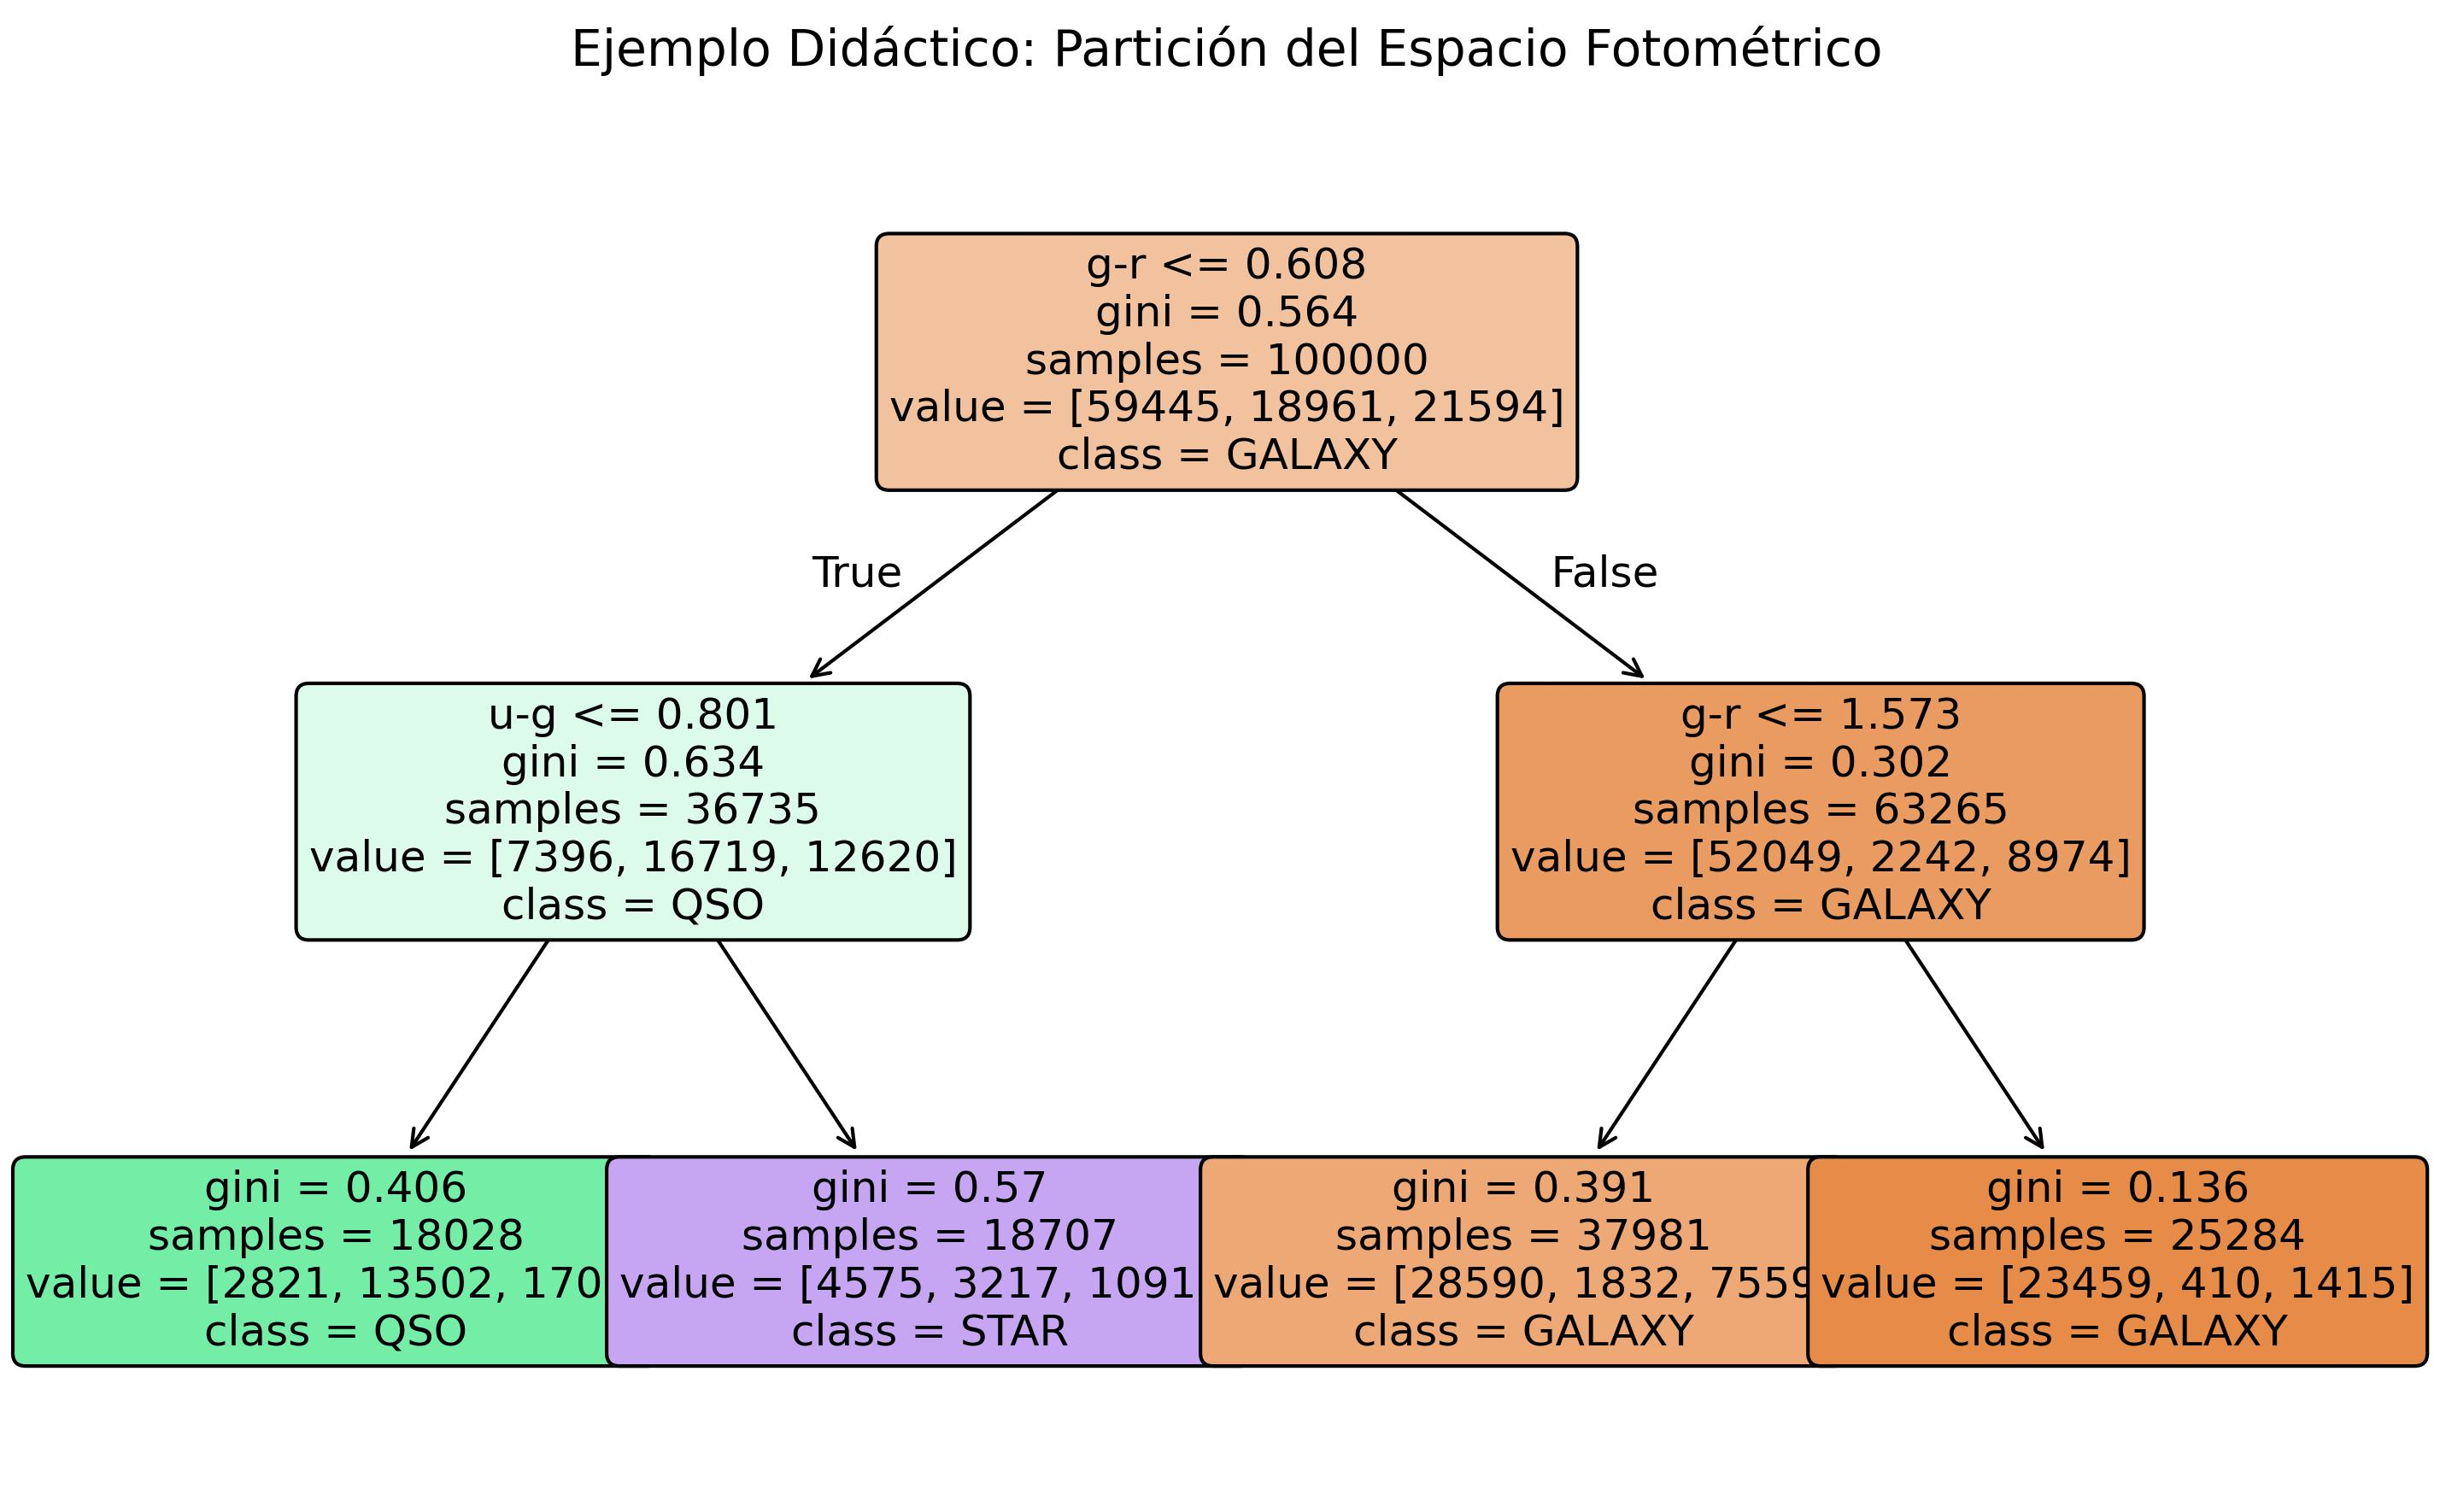
\includegraphics[width=1\textwidth]{arbol_decision_ejemplo.jpg}
    \caption{Ejemplo de un árbol de decisión de profundidad máxima 2, entrenado exclusivamente con los índices de color $u-g$ y $g-r$ del conjunto de datos. El nodo raíz particiona el espacio inicial ($N=100.000$) utilizando el umbral $g-r \leq 0.608$. Se observa visualmente cómo cada división sucesiva reduce el Índice de Gini local, logrando segmentar el espacio fotométrico en regiones dominadas por cuásares (verde), estrellas (morado) y galaxias (naranja).}
    \label{fig:arbol_ejemplo}
\end{figure}


\subsubsection{Ensamblaje de Árboles: El Algoritmo Random Forest}

Aunque los árboles de decisión son modelos altamente interpretables, presentan una deficiencia estadística crítica: poseen una varianza muy elevada y tienden a sobreajustarse a los datos de entrenamiento. Además, si entrenáramos múltiples árboles independientes utilizando las mismas características de entrada, todos tenderían a elegir las mismas variables para sus cortes iniciales. Esto generaría estructuras topológicas casi idénticas, provocando que sus predicciones y errores estuvieran fuertemente correlacionados, lo que anularía los beneficios de promediarlos.

Para solucionar este problema se introduce el algoritmo \textit{Random Forest}. La robustez de Random Forest reside en la aplicación de dos mecanismos estocásticos que decorrelacionan los árboles individuales:

\begin{enumerate}
    \item \textbf{Bagging (\textit{Bootstrap Aggregating}):} Cada árbol $T_b$ del bosque se entrena con una muestra empírica $\mathcal{D}_b$ extraída con reemplazo del conjunto original $\mathcal{D}$ \citep{breiman2001}. Esto permite que aproximadamente un tercio de las muestras no sean vistas por el árbol durante su construcción (las denominadas muestras \textit{Out-Of-Bag}), sirviendo para una validación interna implícita.
    
    \item \textbf{Selección Aleatoria de Características:} En cada división de un nodo, solo se considera un subconjunto aleatorio de $m$ características candidatas ($m < n$). Esto evita que una variable con un alto poder predictivo condicione la estructura de la raíz en todos los árboles, fomentando la diversidad estructural del bosque.
\end{enumerate}

La predicción final del clasificador para una nueva observación se obtiene mediante la agregación de los resultados, utilizando votación mayoritaria entre todos los árboles decorrelacionados que conforman el ensamblaje, tal y como se esquematiza en la Figura \ref{fig:rf_architecture}.


\subsubsection{Importancia de Características}

Una ventaja crucial de Random Forest para la física es su interpretabilidad matemática. La importancia de una característica predictora $X_j$ se calcula sumando la disminución total de impureza ($\Delta Gini$) en todos los nodos $t$ donde se utiliza $X_j$ para realizar la partición, promediado sobre la totalidad de los árboles $N_{trees}$ que componen el bosque:

\begin{equation}
Imp(X_j) = \frac{1}{N_{trees}} \sum_{T} \sum_{t \in T : v(t)=X_j} p(t) \Delta Gini(t)
\label{eq:feature_importance}
\end{equation}

Esta formulación analítica nos permitirá identificar a posteriori qué índices de color fotométrico contienen la mayor cantidad de información física discriminante para la clasificación de los objetos celestes.

% --- FIGURA RF ---   
\begin{figure}[hbt!]
    \centering
    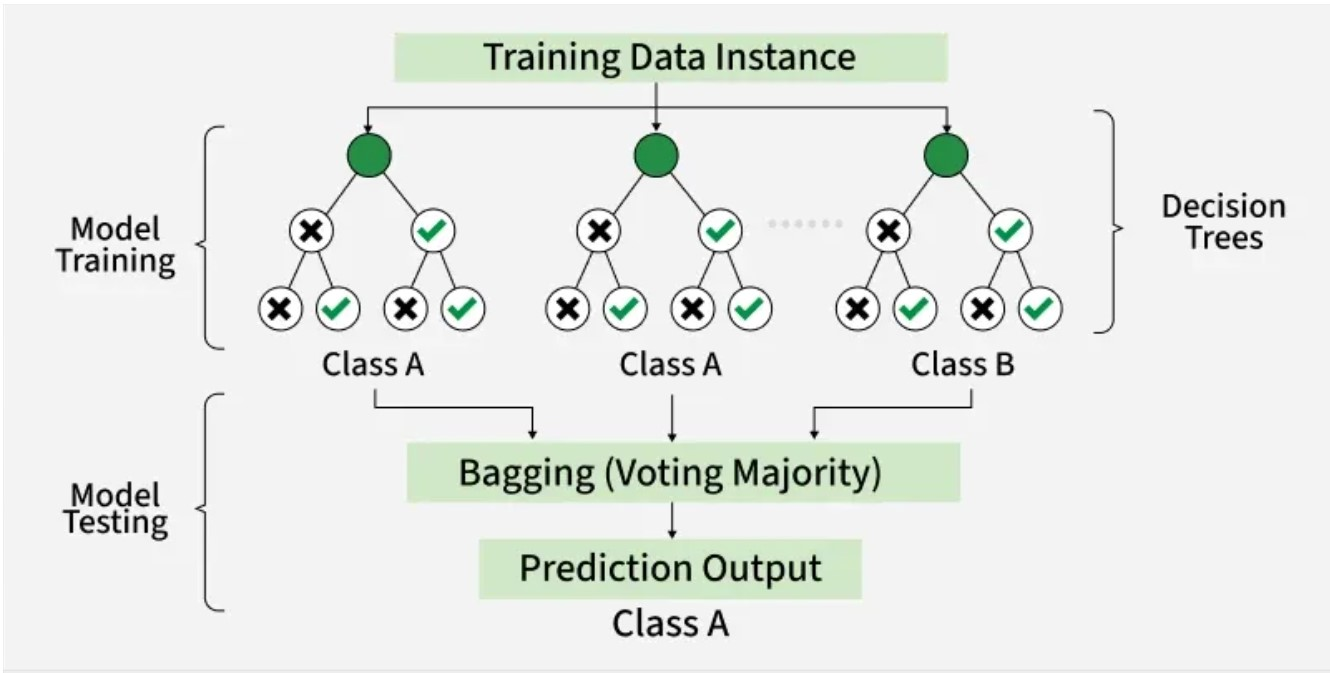
\includegraphics[width=0.8\textwidth]{esquema_rf.jpg} 
    \caption{Arquitectura del modelo Random Forest. Múltiples árboles de decisión operan en paralelo sobre subconjuntos de datos, y la decisión final se toma por votación mayoritaria. Fuente: \url{https://www.geeksforgeeks.org/machine-learning/random-forest-algorithm-in-machine-learning/}}
    \label{fig:rf_architecture}
\end{figure}

\subsection{Máquinas de Vectores de Soporte (SVM)}

Las Máquinas de Vectores de Soporte, introducidas originalmente por \citet{cortes1995}, se fundamentan sólidamente en la teoría del aprendizaje estadístico. Su objetivo analítico es encontrar el hiperplano óptimo que separa las distintas clases en el espacio de características maximizando el \textbf{margen} geométrico, lo que teóricamente garantiza la minimización del límite superior del error de generalización. 

Para establecer este marco teórico de manera progresiva, a continuación se detalla el desarrollo matemático del algoritmo, partiendo de la formulación primal del hiperplano, introduciendo la tolerancia al ruido mediante el margen suave, y culminando con la optimización dual y el truco del kernel para fronteras no lineales. En el desarrollo matemático de toda esta sección se ha utilizado como material de referencia las obras de \citet{hastie2009} y \citet{james2013}.

\subsubsection{Formulación Primal y Margen Suave}

En un escenario ideal bidimensional, supongamos que intentamos separar dos clases (por ejemplo, Estrellas y Galaxias) utilizando únicamente dos índices de color fotométrico, como $r-i$ e $i-z$. Si estos objetos formaran dos grupos perfectamente separables mediante una línea recta, dicha frontera geométrica (el hiperplano) se definiría matemáticamente con la ecuación $\mathbf{w} \cdot \mathbf{x} + b = 0$, donde $\mathbf{w}$ es el vector normal que indica la orientación de la recta y $b$ determina su desplazamiento respecto al origen.

Las observaciones de ambas clases que se sitúan más cerca de esta frontera (los vectores de soporte) dictan la amplitud del \textbf{margen de separación}. Los hiperplanos paralelos que delimitan esta región se sitúan en $\mathbf{w} \cdot \mathbf{x} + b = 1$ para una clase y $\mathbf{w} \cdot \mathbf{x} + b = -1$ para la otra. Dado que la distancia geométrica total entre ambas fronteras es $2 / \|\mathbf{w}\|$, el algoritmo busca maximizar esta anchura resolviendo el problema matemático equivalente de minimizar $\frac{1}{2} \| \mathbf{w} \|^2$.

Sin embargo, los datos fotométricos reales del SDSS rara vez son linealmente separables debido a la dispersión física intrínseca y a las incertidumbres de medición. Siguiendo con el ejemplo, una galaxia lejana con una baja relación señal-ruido podría presentar colores casi idénticos a los de una estrella enana, invadiendo el margen de separación o incluso cruzando al lado equivocado del hiperplano. 

Para gestionar matemáticamente este solapamiento natural, la formulación de Margen Suave (\textit{Soft Margin}) introduce variables de holgura $\xi_i \geq 0$ (\textit{slack variables}). Estas variables actúan como mecanismos de flexibilización que permiten al algoritmo tolerar ciertas invasiones del margen por parte de observaciones anómalas o ruidosas, penalizándolas en la función objetivo en lugar de hacer que el problema matemático sea irresoluble.

El problema de optimización primal se reformula entonces añadiendo esta penalización:
\begin{equation}
    \min_{\mathbf{w}, b, \xi} \left( \frac{1}{2} \|\mathbf{w}\|^2 + C \sum_{i=1}^{m} \xi_i \right)
\end{equation}
Sujeto a las restricciones geométricas relajadas:
\begin{equation}
    y_i (\mathbf{w} \cdot \mathbf{x}_i + b) \geq 1 - \xi_i, \quad \xi_i \geq 0 \quad \forall i
\end{equation}

En esta ecuación, el hiperparámetro de regularización $C > 0$ actúa como el factor de ponderación clave. Un $C$ elevado penaliza severamente cualquier invasión del margen, forzando un ajuste muy estricto a los datos de entrenamiento (con un alto riesgo de sobreajuste o \textit{overfitting}). Por el contrario, un valor reducido de $C$ relaja la penalización, permitiendo un margen de separación más amplio que tolera más observaciones atípicas ($\xi_i > 0$). Esto produce un modelo geométricamente más suave y, a menudo, con mejor capacidad de generalización ante nuevas observaciones.

\subsubsection{Formulación Dual y el "Kernel Trick"}

Para resolver este problema de optimización con restricciones de manera eficiente, y sentar las bases para la separación no lineal, se aplica el método de los Multiplicadores de Lagrange. Esto nos conduce a la formulación dual de Wolfe, que depende exclusivamente de los productos escalares entre las observaciones:
\begin{equation}
    \max_{\alpha} \left( \sum_{i=1}^{m} \alpha_i - \frac{1}{2} \sum_{i,j} \alpha_i \alpha_j y_i y_j K(\mathbf{x}_i, \mathbf{x}_j) \right)
\end{equation}
Sujeto a $0 \leq \alpha_i \leq C$ y $\sum \alpha_i y_i = 0$.

Aquí, $K(\mathbf{x}_i, \mathbf{x}_j) = \phi(\mathbf{x}_i) \cdot \phi(\mathbf{x}_j)$ es la función \textbf{Kernel}. El ``truco del kernel'' (\textit{Kernel Trick}) permite calcular el producto escalar en un espacio de características de alta dimensionalidad $\mathcal{H}$ sin necesidad de computar explícitamente la costosa transformación matemática $\phi$.

En la presente investigación se ha seleccionado el Kernel de Base Radial (RBF) o Gaussiano:
\begin{equation}
    K(\mathbf{x}_i, \mathbf{x}_j) = \exp\left(-\gamma \|\mathbf{x}_i - \mathbf{x}_j\|^2\right)
\end{equation}

La elección empírica del kernel RBF responde a la naturaleza topológica de los datos astronómicos: las poblaciones de estrellas y cuásares no se separan mediante hiperplanos rectos en el espacio de colores del SDSS, sino que forman aglomeraciones o ``nubes'' de densidad complejas. El kernel RBF mapea implícitamente estas observaciones a un espacio de infinitas dimensiones donde sí resultan linealmente separables. 

El hiperparámetro $\gamma$ (gamma) controla el radio de influencia de cada muestra de entrenamiento (vector de soporte). Un $\gamma$ elevado implica que la influencia de una observación es muy local, generando fronteras de decisión cerradas e irregulares alrededor de puntos individuales; mientras que un $\gamma$ bajo extiende dicha influencia, produciendo fronteras de decisión mucho más suaves y continuas.

% --- FIGURA SVM ---
\begin{figure}[hbt!]
    \centering
    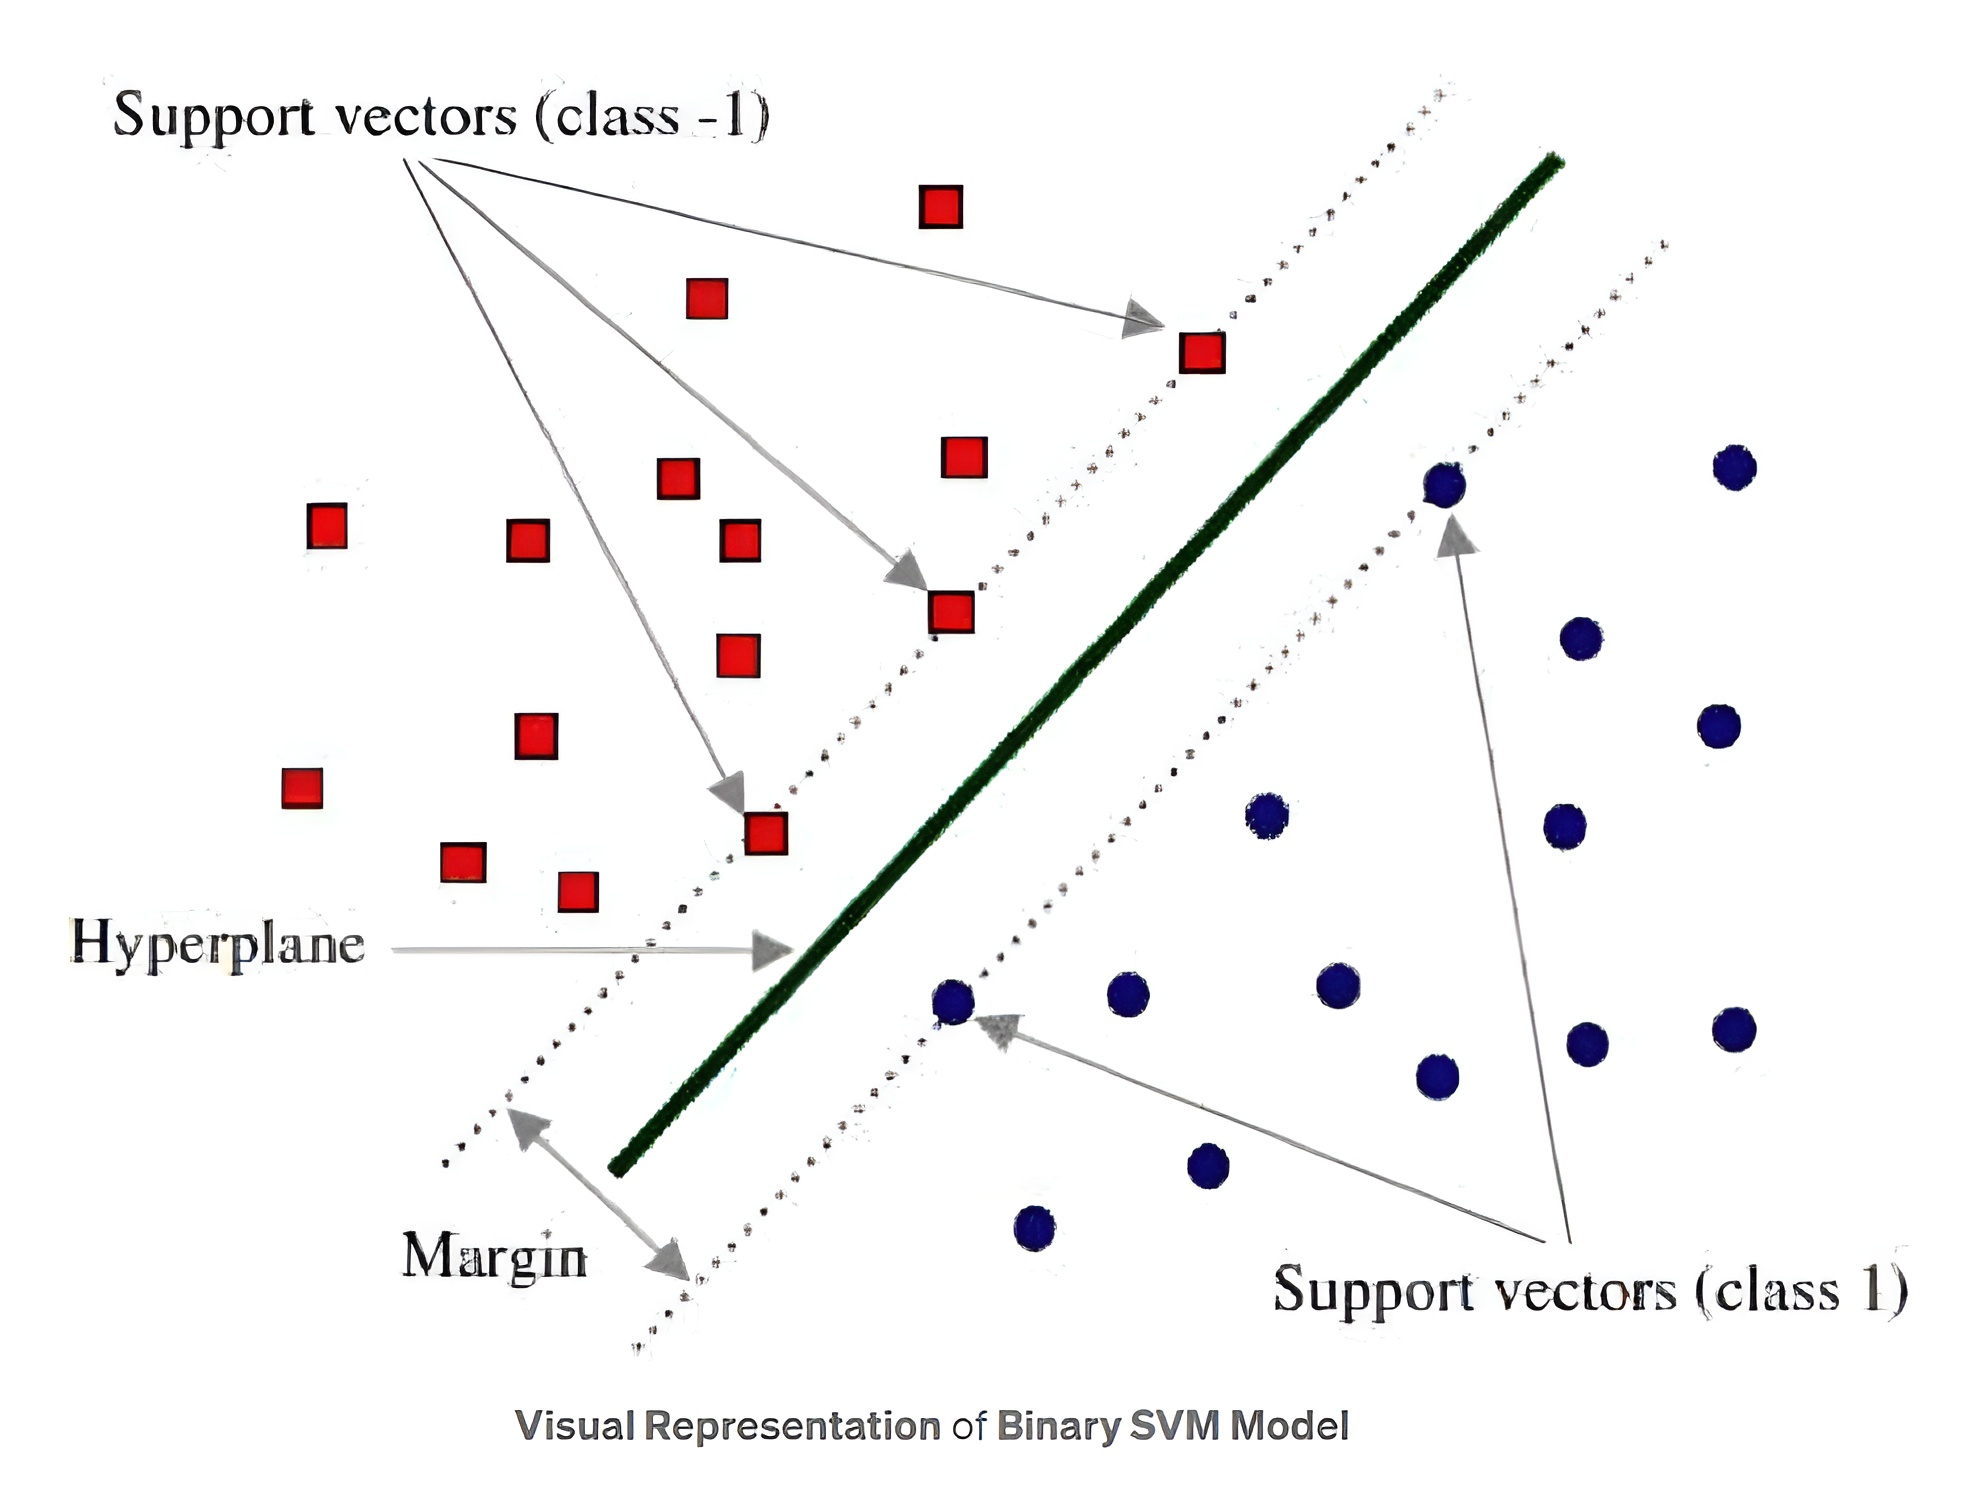
\includegraphics[width=0.6\textwidth]{esquema_svm.jpg}
    \caption{Representación de un SVM binario con margen suave. Los vectores de soporte (puntos rodeados) definen el margen geométrico. Las muestras que violan el margen tienen variables de holgura $\xi_i > 0$. Fuente: \url{https://medium.com/analytics-vidhya/the-svm-we-need-to-know-the-svm-we-implemented-47740d65aa5b}}
    \label{fig:svm_diagram}
\end{figure}
    
\section{Aprendizaje No Supervisado}

En esta aproximación metodológica, los algoritmos operan exclusivamente sobre el espacio de características $\mathcal{X}$ sin acceso a las etiquetas de clase $\mathcal{Y}$. El objetivo analítico es descubrir la estructura latente, la distribución de densidad o la topología intrínseca de los datos empíricos. Para la redacción de esta sección se ha utilizado el siguiente material bibliográfico: \citet{hastie2009}.

\subsection{K-Means Clustering}

El algoritmo K-Means es un método de partición iterativo que busca dividir el conjunto de datos en $K$ agrupaciones disjuntas $C_1, \dots, C_K$, cada una representada por un centroide $\mu_k$.

Matemáticamente, el algoritmo tradicional busca minimizar la inercia o Suma de Errores Cuadráticos (SSE) intra-cluster. Para ello, es necesario definir una métrica de similitud. Aunque en minería de datos se pueden emplear diversas métricas espaciales (como la distancia Manhattan o la similitud del coseno para textos), la formulación estándar de K-Means emplea la distancia Euclídea al cuadrado, ya que es la métrica que se alinea analíticamente con la minimización de la varianza:
\begin{equation}
    \min_{\{\mu_k\}, \{C_k\}} \sum_{k=1}^{K} \sum_{\mathbf{x} \in C_k} \|\mathbf{x} - \mu_k\|^2
\end{equation}

El proceso de optimización clásico es altamente sensible a la posición inicial aleatoria de los centroides, pudiendo converger a mínimos locales subóptimos. Para mitigar esta inestabilidad, en este trabajo se emplea la variante algorítmica \textbf{K-Means++} \citep{arthur2007}. Este método de inicialización probabilística distribuye los primeros centroides lo más alejados posible entre sí, garantizando una convergencia más rápida y robusta.

Una vez inicializados, el algoritmo alterna iterativamente entre dos fases hasta alcanzar la convergencia:
\begin{enumerate}
    \item \textbf{Asignación:} Cada observación $\mathbf{x}$ se asigna al cluster cuyo centroide $\mu_k$ es el más cercano según la distancia Euclídea.
    \item \textbf{Actualización:} Se recalculan los centroides computando la media aritmética (el centro de masas) de los puntos recién asignados a cada cluster.
\end{enumerate}

Al utilizar la distancia Euclídea respecto a un punto central para medir la inercia, el algoritmo asume implícitamente que los clusters tienen una geometría convexa y son isotrópicos (es decir, tienden a formar nubes esféricas con varianza similar en todas las direcciones). Esta característica estructural constituye una limitación fundamental para el problema astrofísico abordado, ya que penaliza enormemente la identificación de las estructuras alargadas, filamentosas o de densidad irregular que típicamente presentan las poblaciones estelares y galácticas en los diagramas color-color.

\subsection{Análisis de Componentes Principales (PCA)}

El Análisis de Componentes Principales o PCA \citep{pearson1901, jolliffe2002} es una técnica matemática de transformación lineal orientada a la reducción de dimensionalidad. Su propósito es mitigar la multicolinealidad entre variables y proyectar los datos originales sobre un nuevo subespacio ortogonal de menor dimensión, de manera que se maximice la varianza retenida de los datos proyectados.

Para evitar que variables con escalas arbitrariamente grandes dominen el modelo de forma artificial, el primer paso riguroso es el centrado de los datos, restando la media empírica de cada característica. Dada esta matriz de datos centrada $\mathbf{X}$ de dimensiones $m \times n$ (donde $m$ son las observaciones y $n$ los índices de color), PCA busca las direcciones de máxima varianza calculando la matriz de covarianza muestral $\mathbf{\Sigma}$:
\begin{equation}
    \mathbf{\Sigma} = \frac{1}{m-1} \mathbf{X}^T \mathbf{X}
\end{equation}

Puesto que $\mathbf{\Sigma}$ es una matriz cuadrada y simétrica, se somete a una descomposición espectral o diagonalización de la forma $\mathbf{\Sigma} \mathbf{v} = \lambda \mathbf{v}$, lo que nos proporciona dos elementos matemáticos clave:
\begin{itemize}
    \item Los \textbf{autovalores} $\lambda_i$, que son escalares que cuantifican la cantidad exacta de varianza explicada por cada nueva componente.
    \item Los \textbf{autovectores} $\mathbf{v}_i$, que son vectores ortogonales que definen las direcciones geométricas de los nuevos ejes en el espacio original (los denominados Componentes Principales).
\end{itemize}

Al ordenar los autovectores de forma descendente según sus autovalores asociados ($\lambda_1 \geq \lambda_2 \geq \dots \geq \lambda_n$), es posible truncar el espacio. Seleccionando únicamente los primeros $d$ componentes que capturen un porcentaje acumulado suficiente de la varianza total (por ejemplo, $>90\%$), se obtiene una representación de dimensionalidad reducida óptima. Esto permite visualizar y procesar la estructura geométrica intrínseca de los datos astronómicos sin sufrir una pérdida significativa de información física.

\section{Métricas de Evaluación y Técnicas de Remuestreo}

Una vez finalizada la fase de entrenamiento de un algoritmo de aprendizaje automático, resulta imperativo cuantificar objetivamente su rendimiento predictivo. La evaluación de un modelo de clasificación consiste en medir su capacidad de generalización ante observaciones no vistas previamente, contrastando sistemáticamente las predicciones emitidas por el algoritmo ($\hat{y}$) frente a las etiquetas reales conocidas ($y$) de un conjunto de prueba independiente.

Sin embargo, la selección de la métrica matemática adecuada para llevar a cabo esta evaluación no es un problema trivial. En contextos donde las clases están fuertemente desbalanceadas, como ocurre habitualmente en los sondeos astronómicos (donde la población de galaxias domina abrumadoramente sobre la de estrellas y cuásares), se requiere el uso de métricas robustas que no se vean sesgadas por la clase mayoritaria ni enmascaren el rendimiento real sobre las clases minoritarias.

La base fundamental para construir todas estas métricas es la \textbf{Matriz de Confusión} $M \in \mathbb{R}^{C \times C}$, donde cada elemento $M_{ij}$ representa el número de observaciones que pertenecen realmente a la clase $i$ pero que fueron predichas por el modelo como clase $j$. Al analizar el rendimiento sobre una clase específica frente al resto (enfoque de clasificación ``uno contra todos'' o \textit{One-vs-Rest}), los resultados se desglosan en cuatro categorías fundamentales: Verdaderos Positivos ($TP$), Verdaderos Negativos ($TN$), Falsos Positivos ($FP$, error de Tipo I) y Falsos Negativos ($FN$, error de Tipo II).

A partir de la extracción de estos valores, se derivan las siguientes métricas de evaluación. Cabe destacar que, al tratarse de un problema multiclase, el subíndice $k$ utilizado en las formulaciones denota que la métrica se está calculando de forma individualizada para una clase específica $k$:

\begin{description}
    \item[Exactitud (Accuracy):] Es la métrica más intuitiva. Representa la proporción global de predicciones correctas sobre el total de observaciones evaluadas.
    \begin{equation}
        \text{Accuracy} = \frac{TP + TN}{TP + TN + FP + FN}
    \end{equation}
    Aunque es útil como medida descriptiva general, en conjuntos de datos fuertemente desbalanceados resulta engañosa (fenómeno conocido como la ``Paradoja de la Exactitud''). Un modelo ingenuo que clasifique sistemáticamente todo como la clase mayoritaria (galaxias) obtendrá una exactitud muy alta, pero será estadísticamente inútil para descubrir objetos raros. Por ello, el análisis exige recurrir a métricas adicionales.

    \item[Precisión (Precision):] Mide la calidad o fiabilidad de las predicciones positivas. Es la proporción de casos positivos reales frente a todos los que el algoritmo ha etiquetado como positivos para la clase $k$. Al penalizar fuertemente los Falsos Positivos ($FP$), evalúa el nivel de ruido del modelo.
    \begin{equation}
        \text{Precision}_k = \frac{TP_k}{TP_k + FP_k}
    \end{equation}
    En nuestro contexto, una alta precisión en la clase cuásar garantiza que cuando el modelo identifica un candidato, existe una altísima probabilidad de que realmente lo sea, minimizando las clasificaciones erróneas.

    \item[Exhaustividad o Sensibilidad (Recall):] Mide la capacidad del modelo para encontrar todos los objetos relevantes de una clase dentro del conjunto de datos. Al penalizar fuertemente los Falsos Negativos ($FN$), es la métrica más crítica para la detección de objetos raros.
    \begin{equation}
        \text{Recall}_k = \frac{TP_k}{TP_k + FN_k}
    \end{equation}
    Para este trabajo, asegurar un alto Recall en las clases estelares significa que el algoritmo no está perdiendo estrellas reales al camuflarlas erróneamente en el fondo masivo de galaxias.

    \item[F1-Score:] Es la media armónica entre la Precisión y la Exhaustividad para la clase $k$. Proporciona una métrica única y balanceada que resume el rendimiento real del clasificador.
    \begin{equation}
        \text{F1}_k = 2 \cdot \frac{\text{Precision}_k \cdot \text{Recall}_k}{\text{Precision}_k + \text{Recall}_k}
    \end{equation}
    A diferencia de la media aritmética, la media armónica penaliza drásticamente los valores extremos. Para que el F1-Score sea alto, tanto la Precisión como el Recall deben ser competitivos, lo que certifica matemáticamente que el modelo no logra su alta sensibilidad a costa de inundar los resultados de falsos positivos.
\end{description}


\subsection{Técnica de Remuestreo: SMOTE}
\label{sec:smote}

Dado que la muestra de estudio presenta un desbalanceo poblacional, con la clase Galaxia con una representación mayoritaria, el entrenamiento estándar de los algoritmos predictivos tiende a sesgarse. Al buscar minimizar la función de coste global, los modelos priorizan el acierto sistemático en la clase mayoritaria, reduciendo la sensibilidad hacia los objetos menos frecuentes. Para mitigar este desequilibrio estructural y evitar que el clasificador desarrolle una frontera de decisión conservadora, en esta investigación se implementa la técnica de remuestreo SMOTE (\textit{Synthetic Minority Over-sampling Technique}), propuesta formalmente por \citet{chawla2002}.

A diferencia de las técnicas de sobremuestreo aleatorio tradicional (\textit{Random Oversampling}), que consisten en la mera duplicación exacta de las observaciones minoritarias, SMOTE aporta información topológica nueva al modelo. La duplicación simple no incrementa la varianza de la clase; geométricamente, solo aumenta la "masa" de puntos específicos, lo que provoca que algoritmos no lineales (como Support Vector Machines o Random Forest) dibujen fronteras de decisión extremadamente cerradas y específicas alrededor de esas coordenadas, incurriendo en un severo sobreajuste o \textit{overfitting} \citep{he2009}. 

Para evitar este fenómeno, SMOTE opera de forma heurística densificando la región de la clase minoritaria mediante la generación de muestras sintéticas genuinas en el espacio continuo de características. Matemáticamente, para una observación $\mathbf{x}_i$ perteneciente a la clase minoritaria, el algoritmo identifica sus $k$ vecinos más cercanos (típicamente empleando $k=5$) dentro de su misma distribución taxonómica, evaluando la proximidad mediante la distancia euclídea. 

A continuación, selecciona aleatoriamente uno de estos vecinos, denotado como $\mathbf{x}_{vecino}$, e interpola un nuevo vector sintético a lo largo del segmento de recta hiperdimensional que los une:
\begin{equation}
    \mathbf{x}_{new} = \mathbf{x}_i + \delta \cdot (\mathbf{x}_{vecino} - \mathbf{x}_i)
\end{equation}
Donde $\delta \sim U(0,1)$ es un número escalar aleatorio extraído de una distribución uniforme continua entre 0 y 1. 

Es fundamental destacar la idoneidad de esta formulación matemática para el presente estudio. Si bien la técnica SMOTE puede introducir ruido en conjuntos de datos con variables categóricas complejas, en el contexto puramente fotométrico de este trabajo resulta excepcionalmente robusta. Al estar nuestro espacio de características compuesto exclusivamente por variables continuas (índices de color y \textit{redshift}), las combinaciones lineales convexas de objetos celestes reales generan firmas espectrales sintéticas físicamente plausibles. Estos nuevos vectores no son anomalías, sino que caen de manera natural dentro de los límites térmicos reales de las distribuciones, rellenando las regiones dispersas de la variedad de la clase minoritaria sin desvirtuar su naturaleza astrofísica.

Finalmente, es necesario puntualizar que, para preservar la rigurosidad analítica y evitar el sesgo por fuga de información (\textit{data leakage}), la técnica SMOTE se aplica de forma estricta y exclusiva sobre el conjunto de entrenamiento (\textit{Training set}) tras la partición estratificada inicial. El conjunto de prueba (\textit{Test set}) se mantiene completamente inalterado, conservando la distribución poblacional y el desbalanceo real del catálogo original. Esto garantiza que las métricas de evaluación posteriores reflejen de manera honesta y realista la capacidad de generalización del modelo ante nuevas detecciones astronómicas.

% --- FIGURA SMOTE ---
\begin{figure}[hbt!]
    \centering
    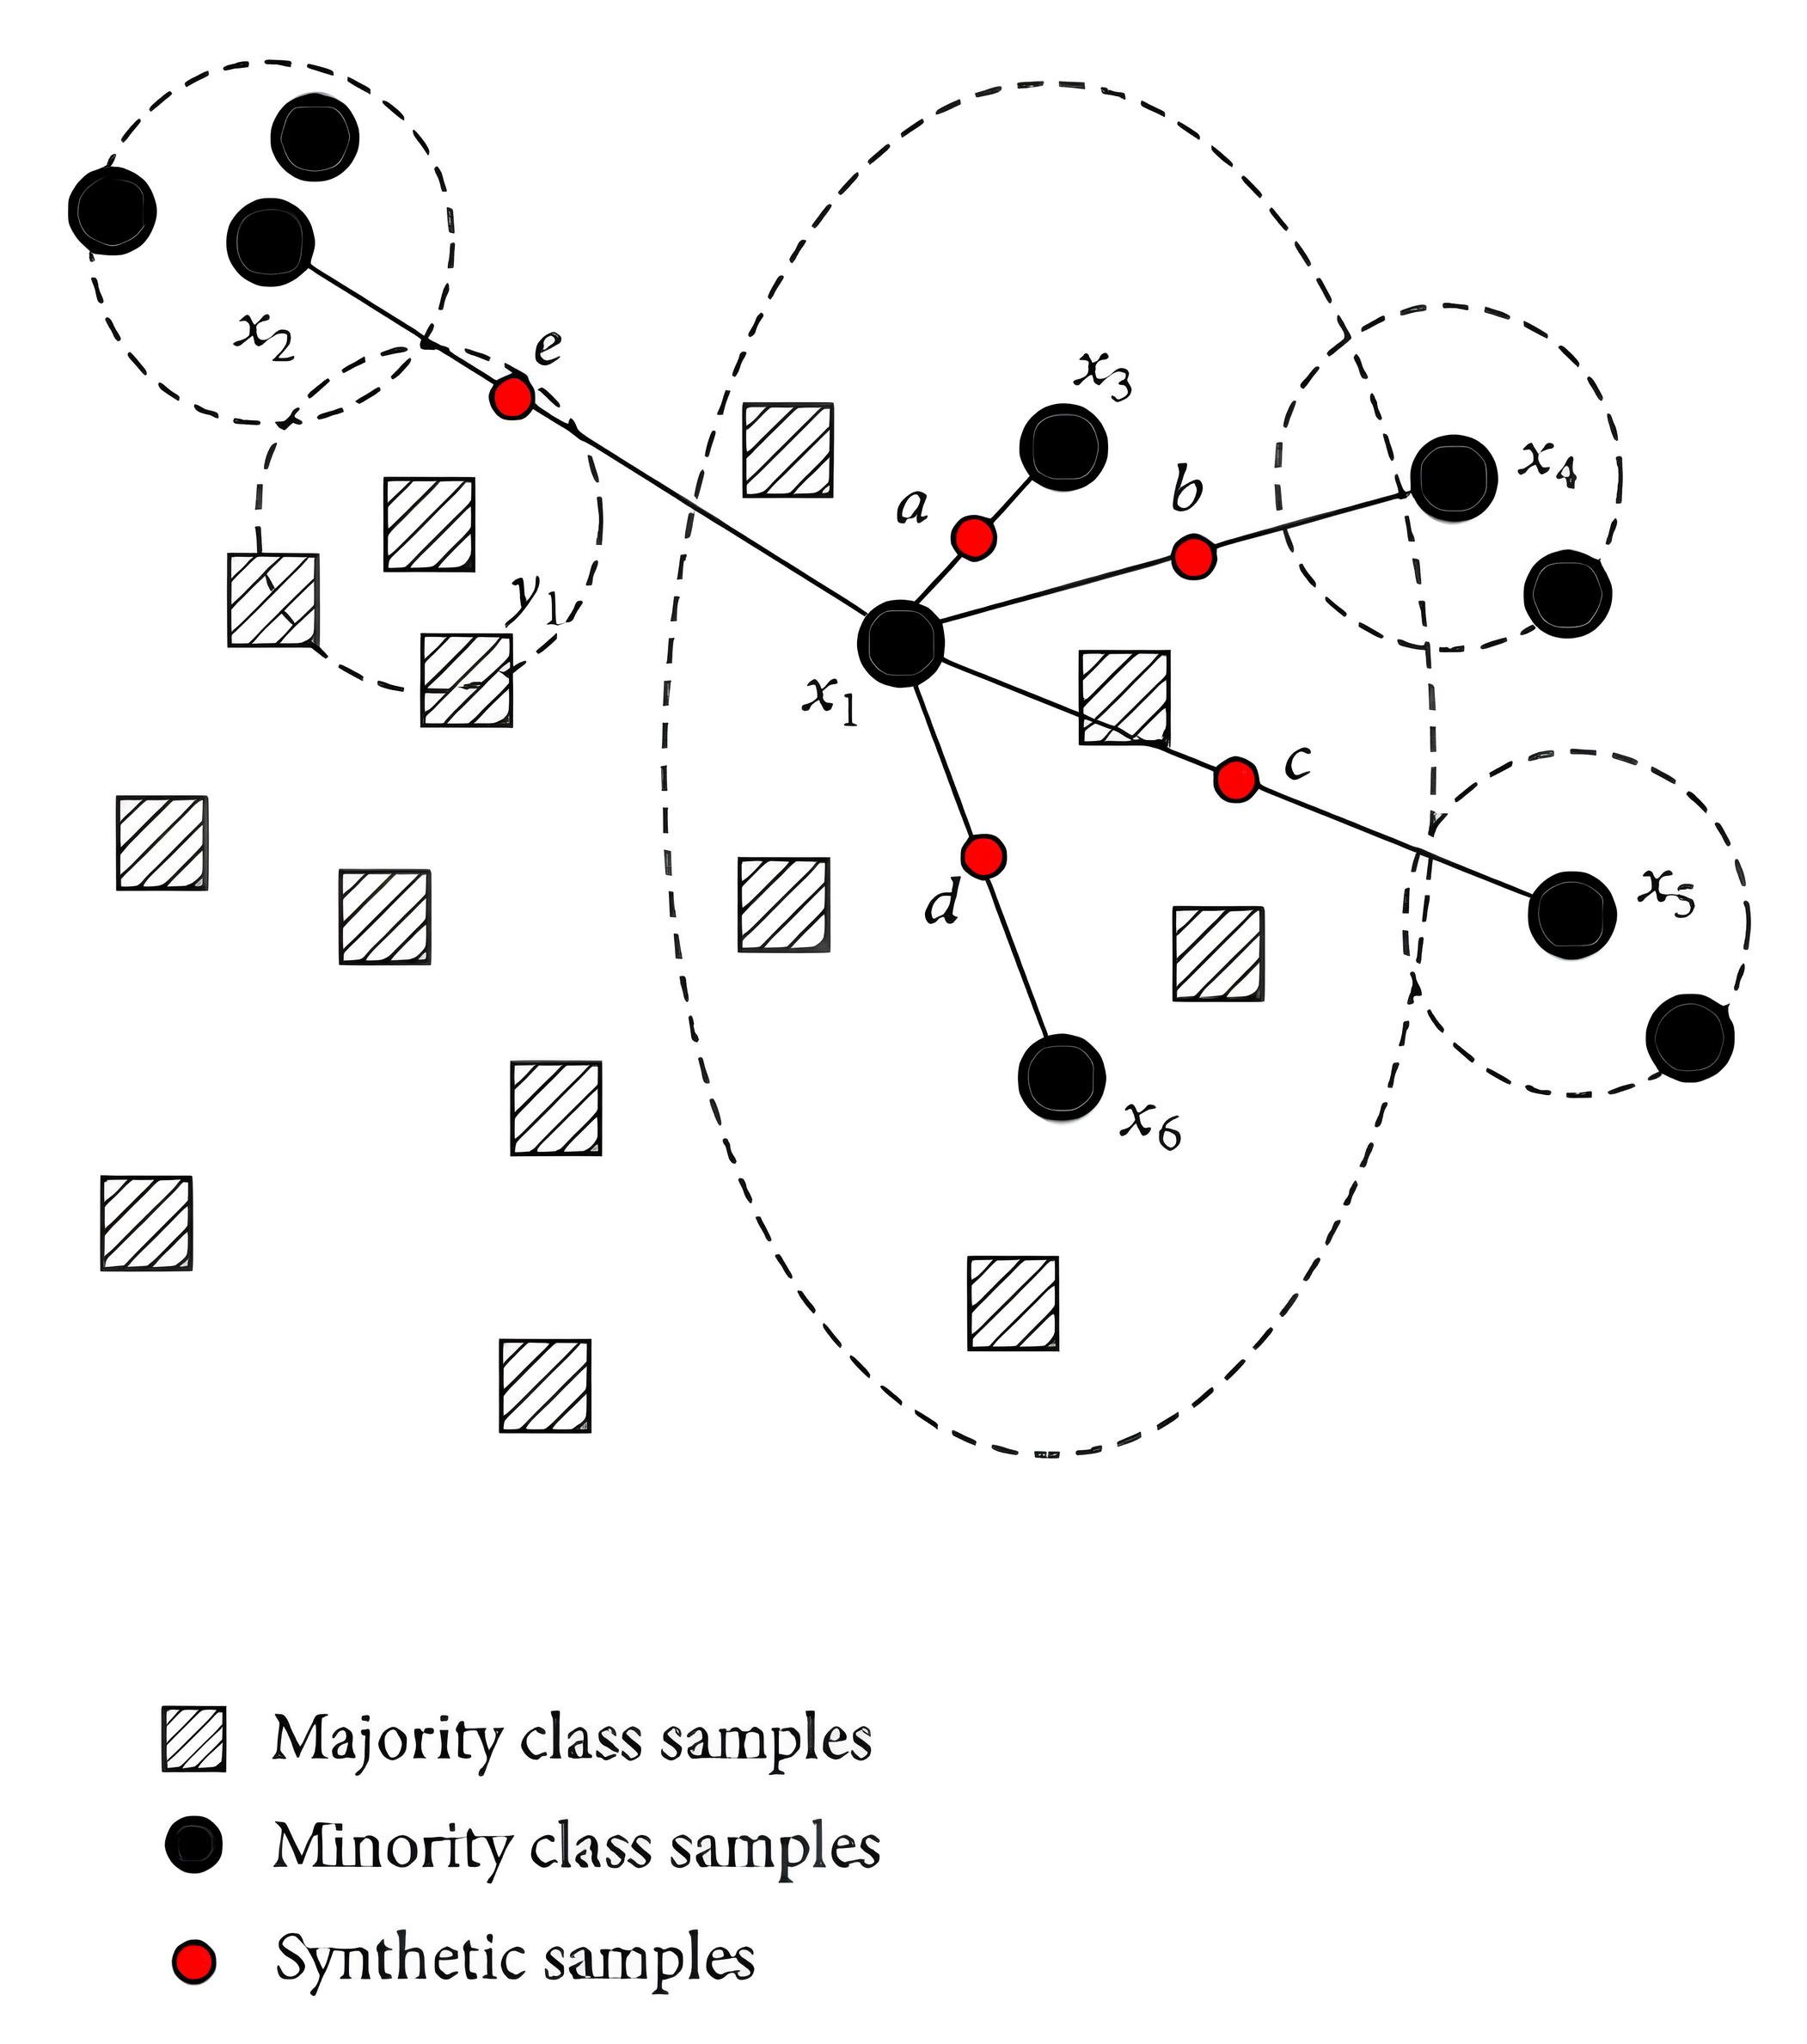
\includegraphics[width=0.8\textwidth]{esquema_smote.jpg}
    \caption{Funcionamiento geométrico del algoritmo SMOTE. En lugar de duplicar puntos empíricos (lo que causaría sobreajuste), el algoritmo identifica los vecinos más cercanos en el espacio continuo de características y genera nuevas observaciones sintéticas interpolando a lo largo de los segmentos que los conectan. Al aplicarse sobre variables fotométricas continuas, los puntos resultantes mantienen plena coherencia física. Imagen adaptada de \citet{rida2019}.}
    \label{fig:smote_diagram}
\end{figure}

%---------------------------------------------------------------------
% CAPÍTULO 3
\chapter{Metodología y Tratamiento de Datos}
\label{chap:metodologia}
%---------------------------------------------------------------------

La calidad de un modelo de aprendizaje automático depende intrínsecamente de la calidad de los datos utilizados. En este capítulo se detalla la procedencia de los datos, el proceso de limpieza y, fundamentalmente, la ingeniería de características basada en principios físicos que permite transformar las magnitudes observadas en variables discriminantes eficaces.

\section{Fuente de Datos: Sloan Digital Sky Survey (SDSS)}

Los datos utilizados en este trabajo provienen del \textit{Sloan Digital Sky Survey} (SDSS), específicamente de su \textit{Data Release 17} (DR17) \citep{Abdurrouf2022}, el cual utiliza un telescopio óptico de 2.5 metros de gran campo situado en el Observatorio de Apache Point (Nuevo México).

La característica fundamental de este sondeo es su sistema fotométrico, que observa el cielo a través de cinco filtros de banda ancha ($u, g, r, i, z$), cubriendo desde el espectro visible hasta el infrarrojo cercano. Las especificaciones técnicas de estos filtros y su correspondencia con el espectro óptico se detallan en la Tabla \ref{tab:filtros_sdss}. La respuesta espectral de estos filtros, que determina qué tipo de información física capturamos de los objetos celestes, se puede observar en las curvas de eficiencia cuántica de la Figura \ref{fig:sdss_filters}.

\begin{table}[hbt!]
\centering
\small 
\begin{tabular}{|c|c|p{8.5cm}|}
\hline
\textbf{Filtro} & \textbf{Longitud de Onda (\AA)} & \textbf{Descripción Física} \\ \hline
$u$ & 3543 & Azul. Sensible a propiedades térmicas altas y líneas de emisión. \\ \hline
$g$ & 4770 & Verde. Parte visible del espectro. \\ \hline
$r$ & 6231 & Rojo. Sensible a la emisión H-alfa. \\ \hline
$i$ & 7625 & Infrarrojo Cercano 1. \\ \hline
$z$ & 9134 & Infrarrojo Cercano 2. \\ \hline
\end{tabular}
\caption{Especificaciones del sistema fotométrico del SDSS. Las longitudes de onda cubren el rango óptico esencial para la clasificación estelar y galáctica.}
\label{tab:filtros_sdss}
\end{table}

% --- IMAGEN: Curvas de respuesta ---
\begin{figure}[H]
    \centering
    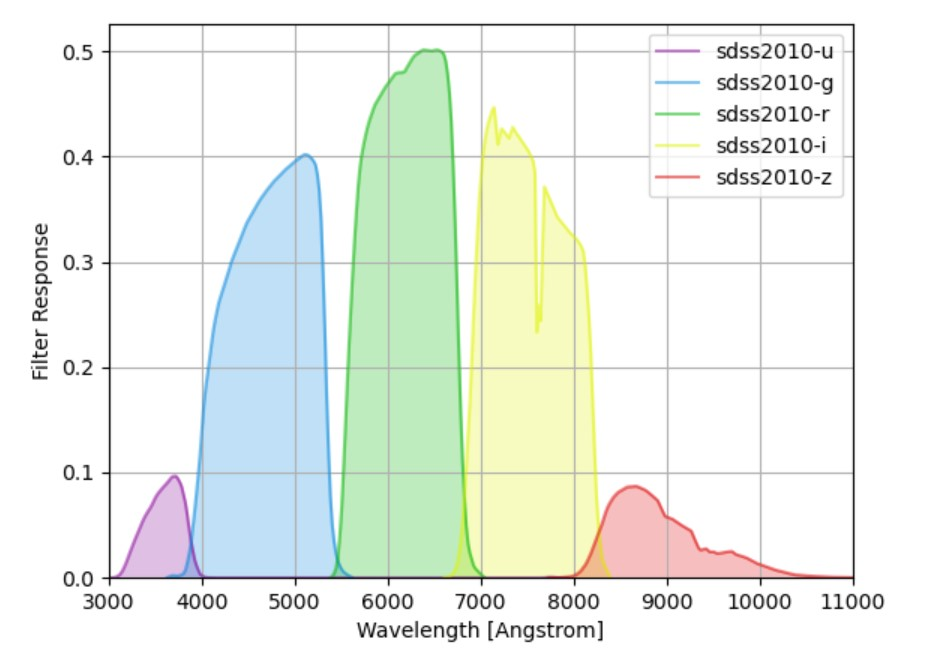
\includegraphics[width=0.8\textwidth]{sdss_filters.jpg} 
    \caption{Curvas de eficiencia cuántica total para los cinco filtros del sistema fotométrico del SDSS. Se muestra el modelo de respuesta estándar \citep{doi2010}, representativo de la instrumentación utilizada para obtener los datos del DR17.}
    \label{fig:sdss_filters}
\end{figure}

La muestra seleccionada consta inicialmente de 100.000 observaciones clasificadas espectroscópicamente, obtenidas a través del repositorio de datos estructurados de Kaggle \citep{kaggle_sdss17}. Cada registro cuenta con los parámetros descritos en la Tabla \ref{tab:parametros_dataset}.

\begin{table}[H]
\centering
\begin{tabular}{ll}
\hline
\textbf{Variable} & \textbf{Descripción} \\ \hline
\texttt{u, g, r, i, z} & Magnitudes fotométricas aparentes en cada filtro del sistema SDSS. \\
\texttt{redshift} & Corrimiento al rojo espectroscópico (medida de distancia/velocidad). \\
\texttt{class} & Variable objetivo categórica (GALAXY, STAR, QSO). \\ \hline
\end{tabular}
\caption{Principales parámetros del conjunto de datos utilizado para la clasificación.}
\label{tab:parametros_dataset}
\end{table}

Los objetos se dividen en tres categorías principales:
\begin{itemize}
    \item \textbf{GALAXY:} Galaxias (objetos extensos y resueltos).
    \item \textbf{STAR:} Estrellas (objetos puntuales pertenecientes a la Vía Láctea).
    \item \textbf{QSO:} Cuásares (núcleos galácticos activos, objetos cuasi-estelares distantes).
\end{itemize}

Como se observa en la Figura \ref{fig:distribucion}, el conjunto presenta un fuerte desbalanceo de clases, lo cual condiciona la elección de métricas de evaluación y motiva el uso de la técnica de remuestreo SMOTE en la fase experimental.

% --- IMAGEN DE DISTRIBUCIÓN ---
\begin{figure}[H]
    \centering
    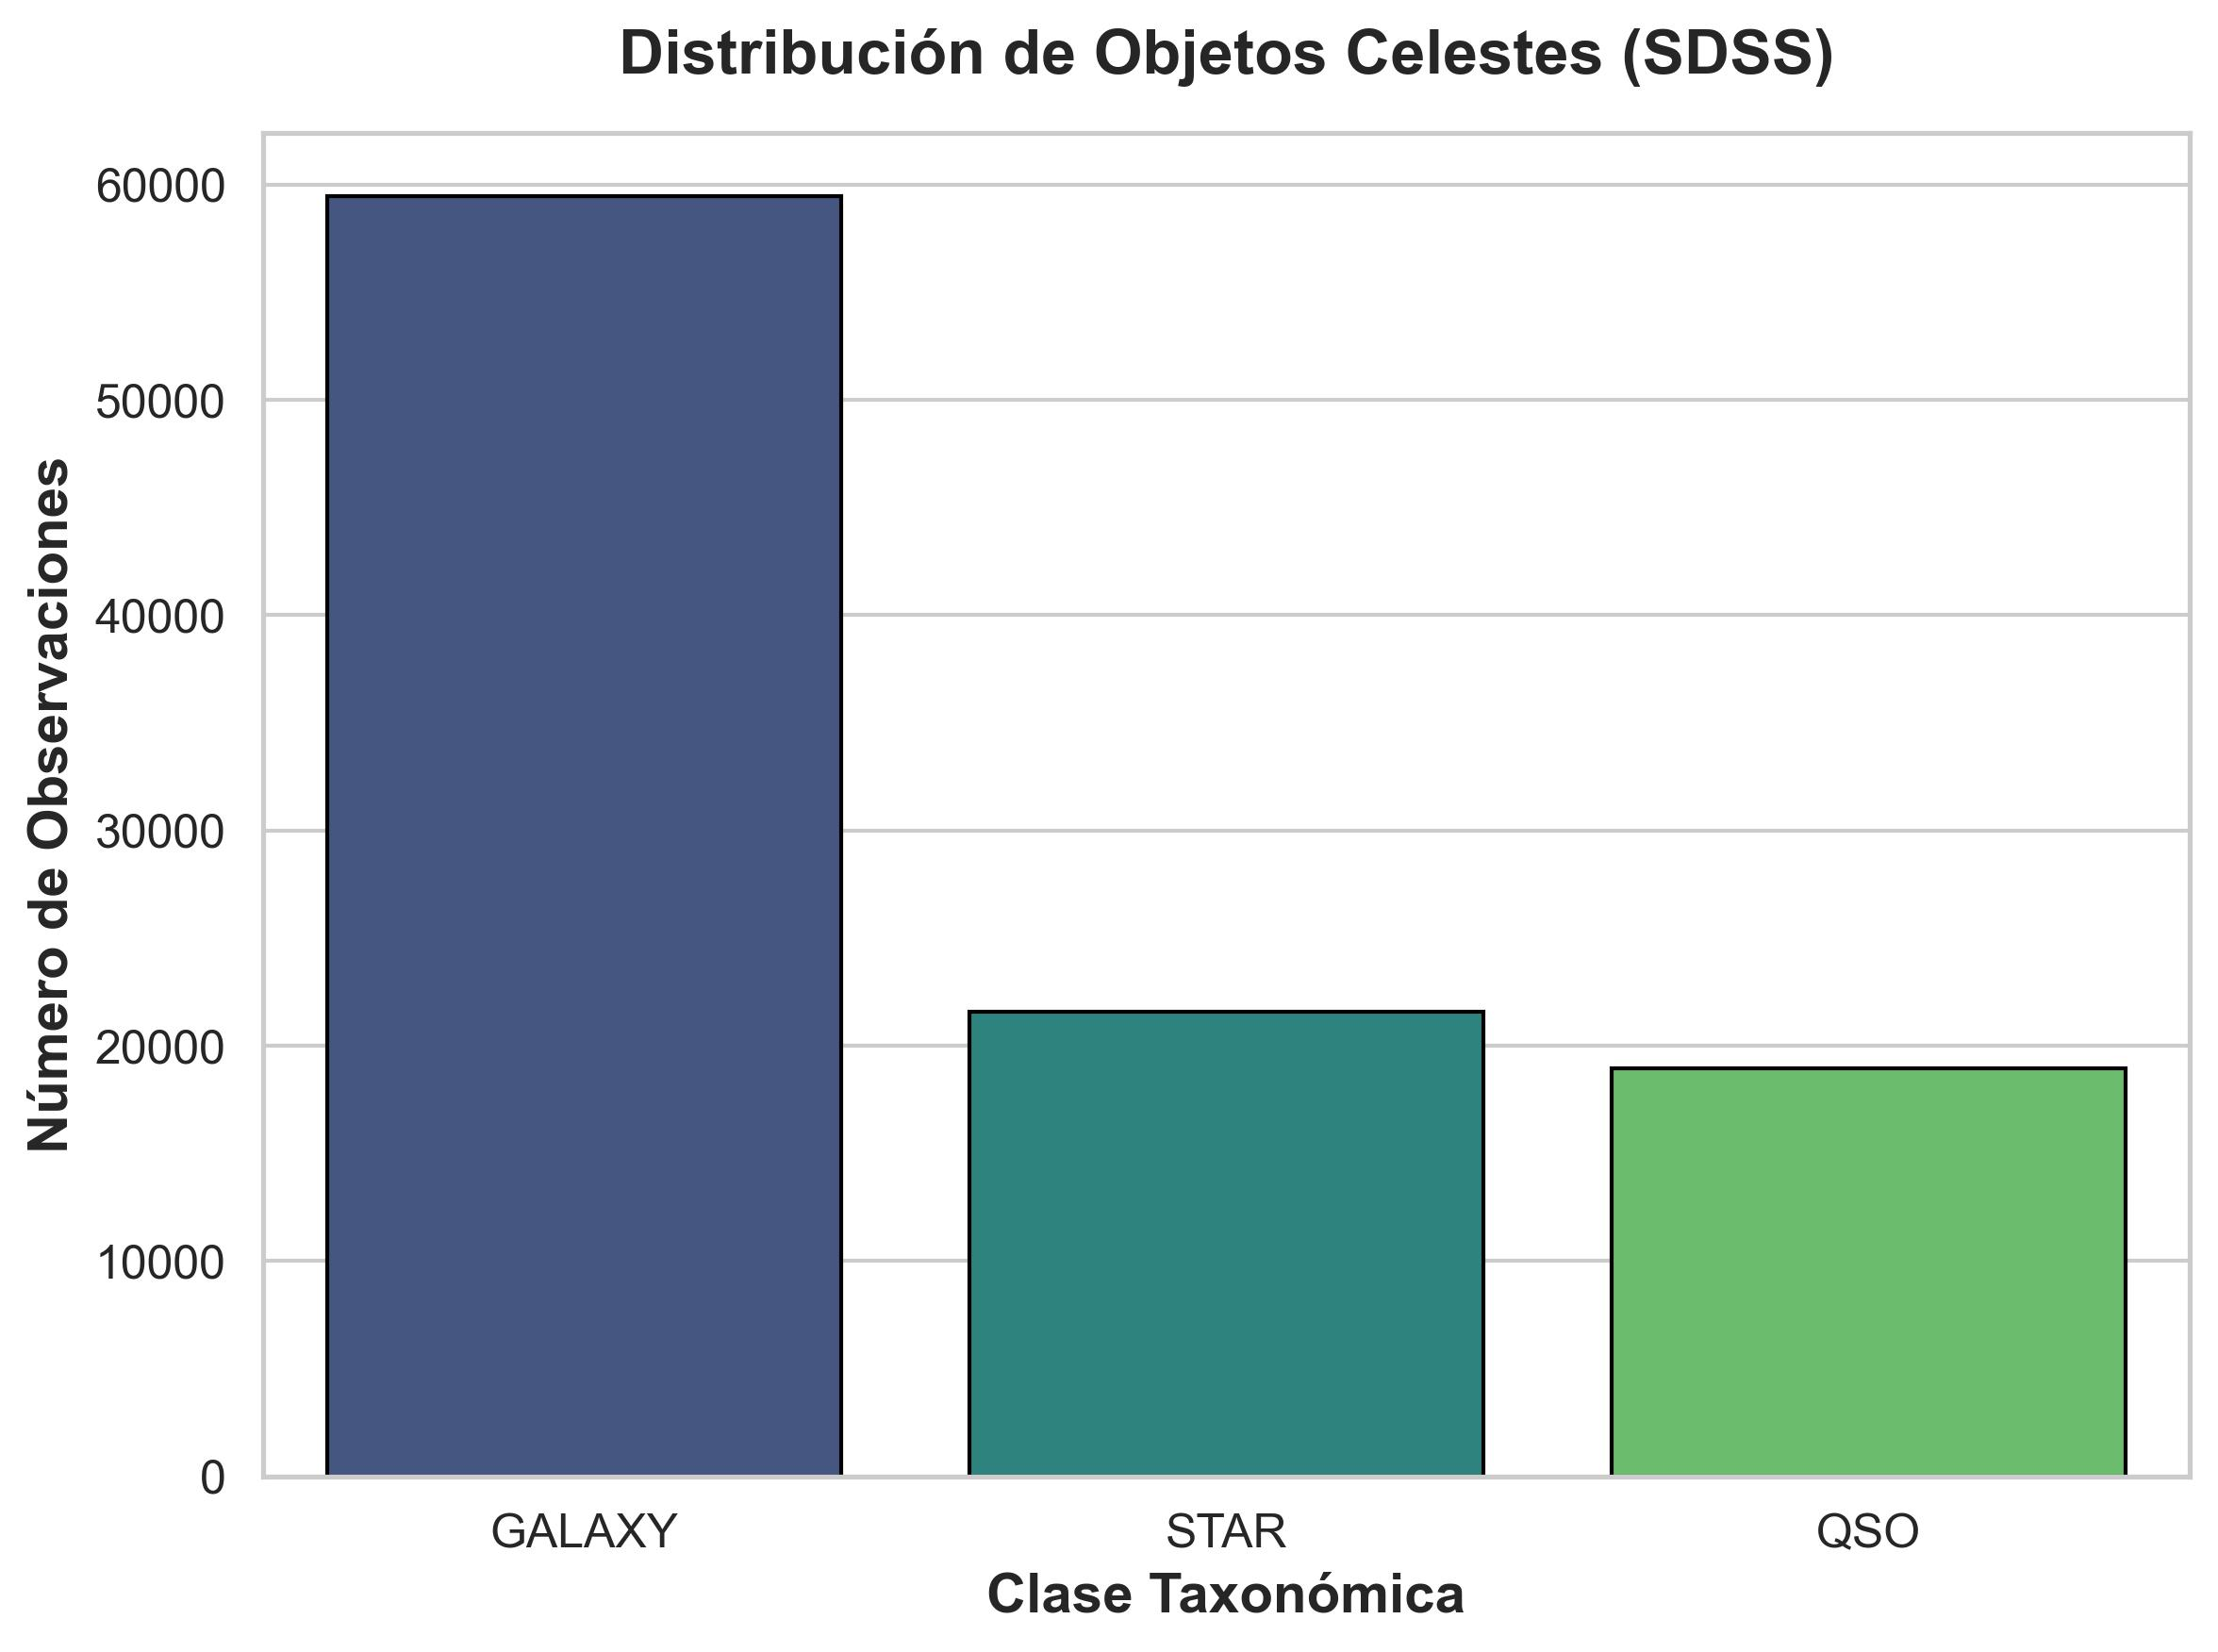
\includegraphics[width=0.8\textwidth]{1_distribucion_clases.jpg}
    \caption{Distribución de clases en el conjunto de datos SDSS. Existe un claro predominio poblacional de las Galaxias frente a las Estrellas y Cuásares.}
    \label{fig:distribucion}
\end{figure}

\section{Preprocesamiento de los Datos}

Antes de aplicar cualquier algoritmo, se realizó una auditoría de calidad de los datos. Esta práctica es un estándar metodológico fundamental en la Minería de Datos \citep{orallo2004, maimon2010} para evitar que el modelo asimile ruido instrumental como si fuera información física real.

Se aplicó un filtro de limpieza riguroso para eliminar registros con valores anómalos (como magnitudes registradas como $-9999$), que corresponden a errores de saturación en el detector CCD o fallos en el proceso de reducción de los datos del SDSS. En nuestra muestra empírica original de 100.000 registros, se detectó y eliminó exactamente 1 observación anómala (perteneciente a la clase \texttt{STAR}) con estas características, generando un conjunto limpio y definitivo de 99.999 muestras útiles.

\section{Ingeniería de Características: Magnitudes vs. Colores}
\label{sec:ingenieria_caracteristicas}

El conjunto de datos original ofrece las magnitudes fotométricas observadas ($u, g, r, i, z$). Utilizar estos valores directamente introduciría un sesgo físico indeseado en los algoritmos: el brillo aparente de un objeto depende intrínsecamente de la distancia a la que se encuentre el observador \citep{ivezic2014}. 

En astronomía, la magnitud aparente $m$ es una función logarítmica del flujo de energía detectado $F$, definida como $m = -2.5 \log_{10}(F) + C$. A su vez, el flujo obedece a la ley de la inversa del cuadrado de la distancia ($F = L / 4\pi d^2$), donde $L$ es la luminosidad intrínseca y $d$ la distancia.

Siguiendo la recomendación metodológica de trabajar con variables independientes de la distancia, se transformó el espacio de características original a un \textbf{espacio de color} mediante la diferencia de magnitudes entre bandas adyacentes (por ejemplo, $u-g$). Matemáticamente, al restar dos magnitudes, se obtiene el cociente de sus flujos:
\begin{equation}
    u - g = -2.5 \log_{10}(F_u) - \left(-2.5 \log_{10}(F_g)\right) = -2.5 \log_{10}\left(\frac{F_u}{F_g}\right)
\end{equation}

Sustituyendo el flujo por su relación geométrica, observamos la cancelación exacta del factor de distancia:
\begin{equation}
    u - g = -2.5 \log_{10}\left( \frac{L_u / 4\pi d^2}{L_g / 4\pi d^2} \right) = -2.5 \log_{10}\left(\frac{L_u}{L_g}\right)
\end{equation}

Esta operación matemática tiene consecuencias físicas vitales:
\begin{enumerate}
    \item \textbf{Cancelación de la Distancia Geométrica:} Como demuestra la ecuación anterior, el color depende únicamente del cociente de las luminosidades intrínsecas ($L_u/L_g$), eliminando el sesgo espacial $1/d^2$.
    \item \textbf{Caracterización Espectral:} El color captura directamente la pendiente del espectro. Mientras que las estrellas térmicas se agrupan en una región cinemática estrecha y bien definida conocida como \textit{Stellar Locus}, los cuásares presentan una emisión no térmica (ley de potencias) proveniente de su disco de acreción. Esto genera un característico ``exceso ultravioleta'' en la banda $u$ que los sitúa completamente fuera del locus estelar \citep{richards2001}.
\end{enumerate}

Como se observa en la Figura \ref{fig:espacios}, esta transformación resulta determinante. En el espacio original (izquierda), las clases se solapan debido a la degeneración por distancia (estrellas débiles y galaxias lejanas pueden tener el mismo brillo aparente). En el espacio de color (derecha), la separación obedece puramente a propiedades intrínsecas (temperatura y morfología espectral), facilitando el hallazgo de hiperplanos de separación para los algoritmos, aunque sigue habiendo solapamientos.

% --- FIGURA DE MAGNITUDES VS COLORES ---
\begin{figure}[hbt!]
    \centering
    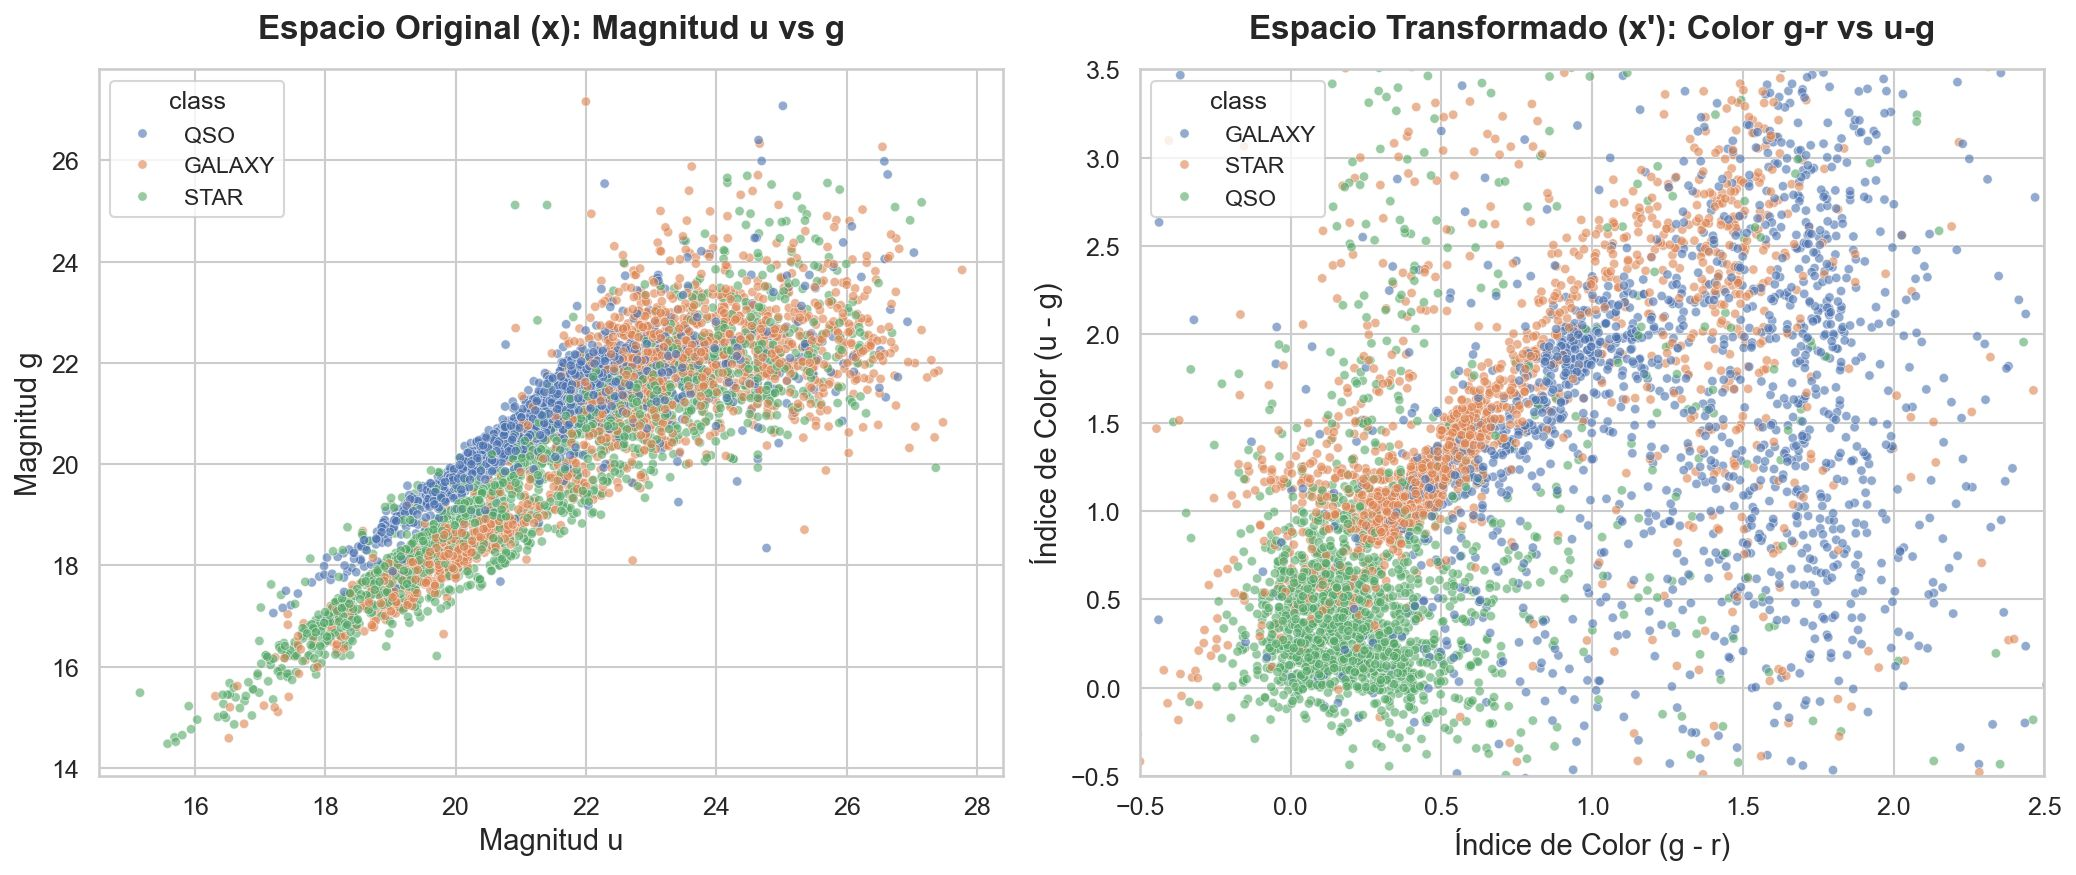
\includegraphics[width=\textwidth]{4_comparativa_espacios.jpg}
    \caption{Panel comparativo de la transformación del espacio de características. A la izquierda, el espacio original definido por las magnitudes aparentes observadas ($u$ frente a $g$), donde se aprecia un severo solapamiento topológico entre clases. Esta mezcla poblacional está provocada por la degeneración geométrica de la distancia, ya que objetos intrínsecamente débiles y cercanos se confunden con objetos muy luminosos y lejanos. A la derecha, el espacio transformado mediante índices de color ($u-g$ frente a $g-r$). Al realizar la resta de magnitudes, se cancela analíticamente la dependencia espacial inversa al cuadrado, revelando exclusivamente las propiedades termodinámicas y espectrales de las fuentes. En esta proyección se hace evidente la formación de la secuencia principal (\textit{Stellar Locus}) y su separación geométrica respecto a la nube de cuásares.}
    \label{fig:espacios}
\end{figure}

% --- FIGURA NUEVA: STELLAR LOCUS VS QUASARS ---
\begin{figure}[hbt!]
    \centering
    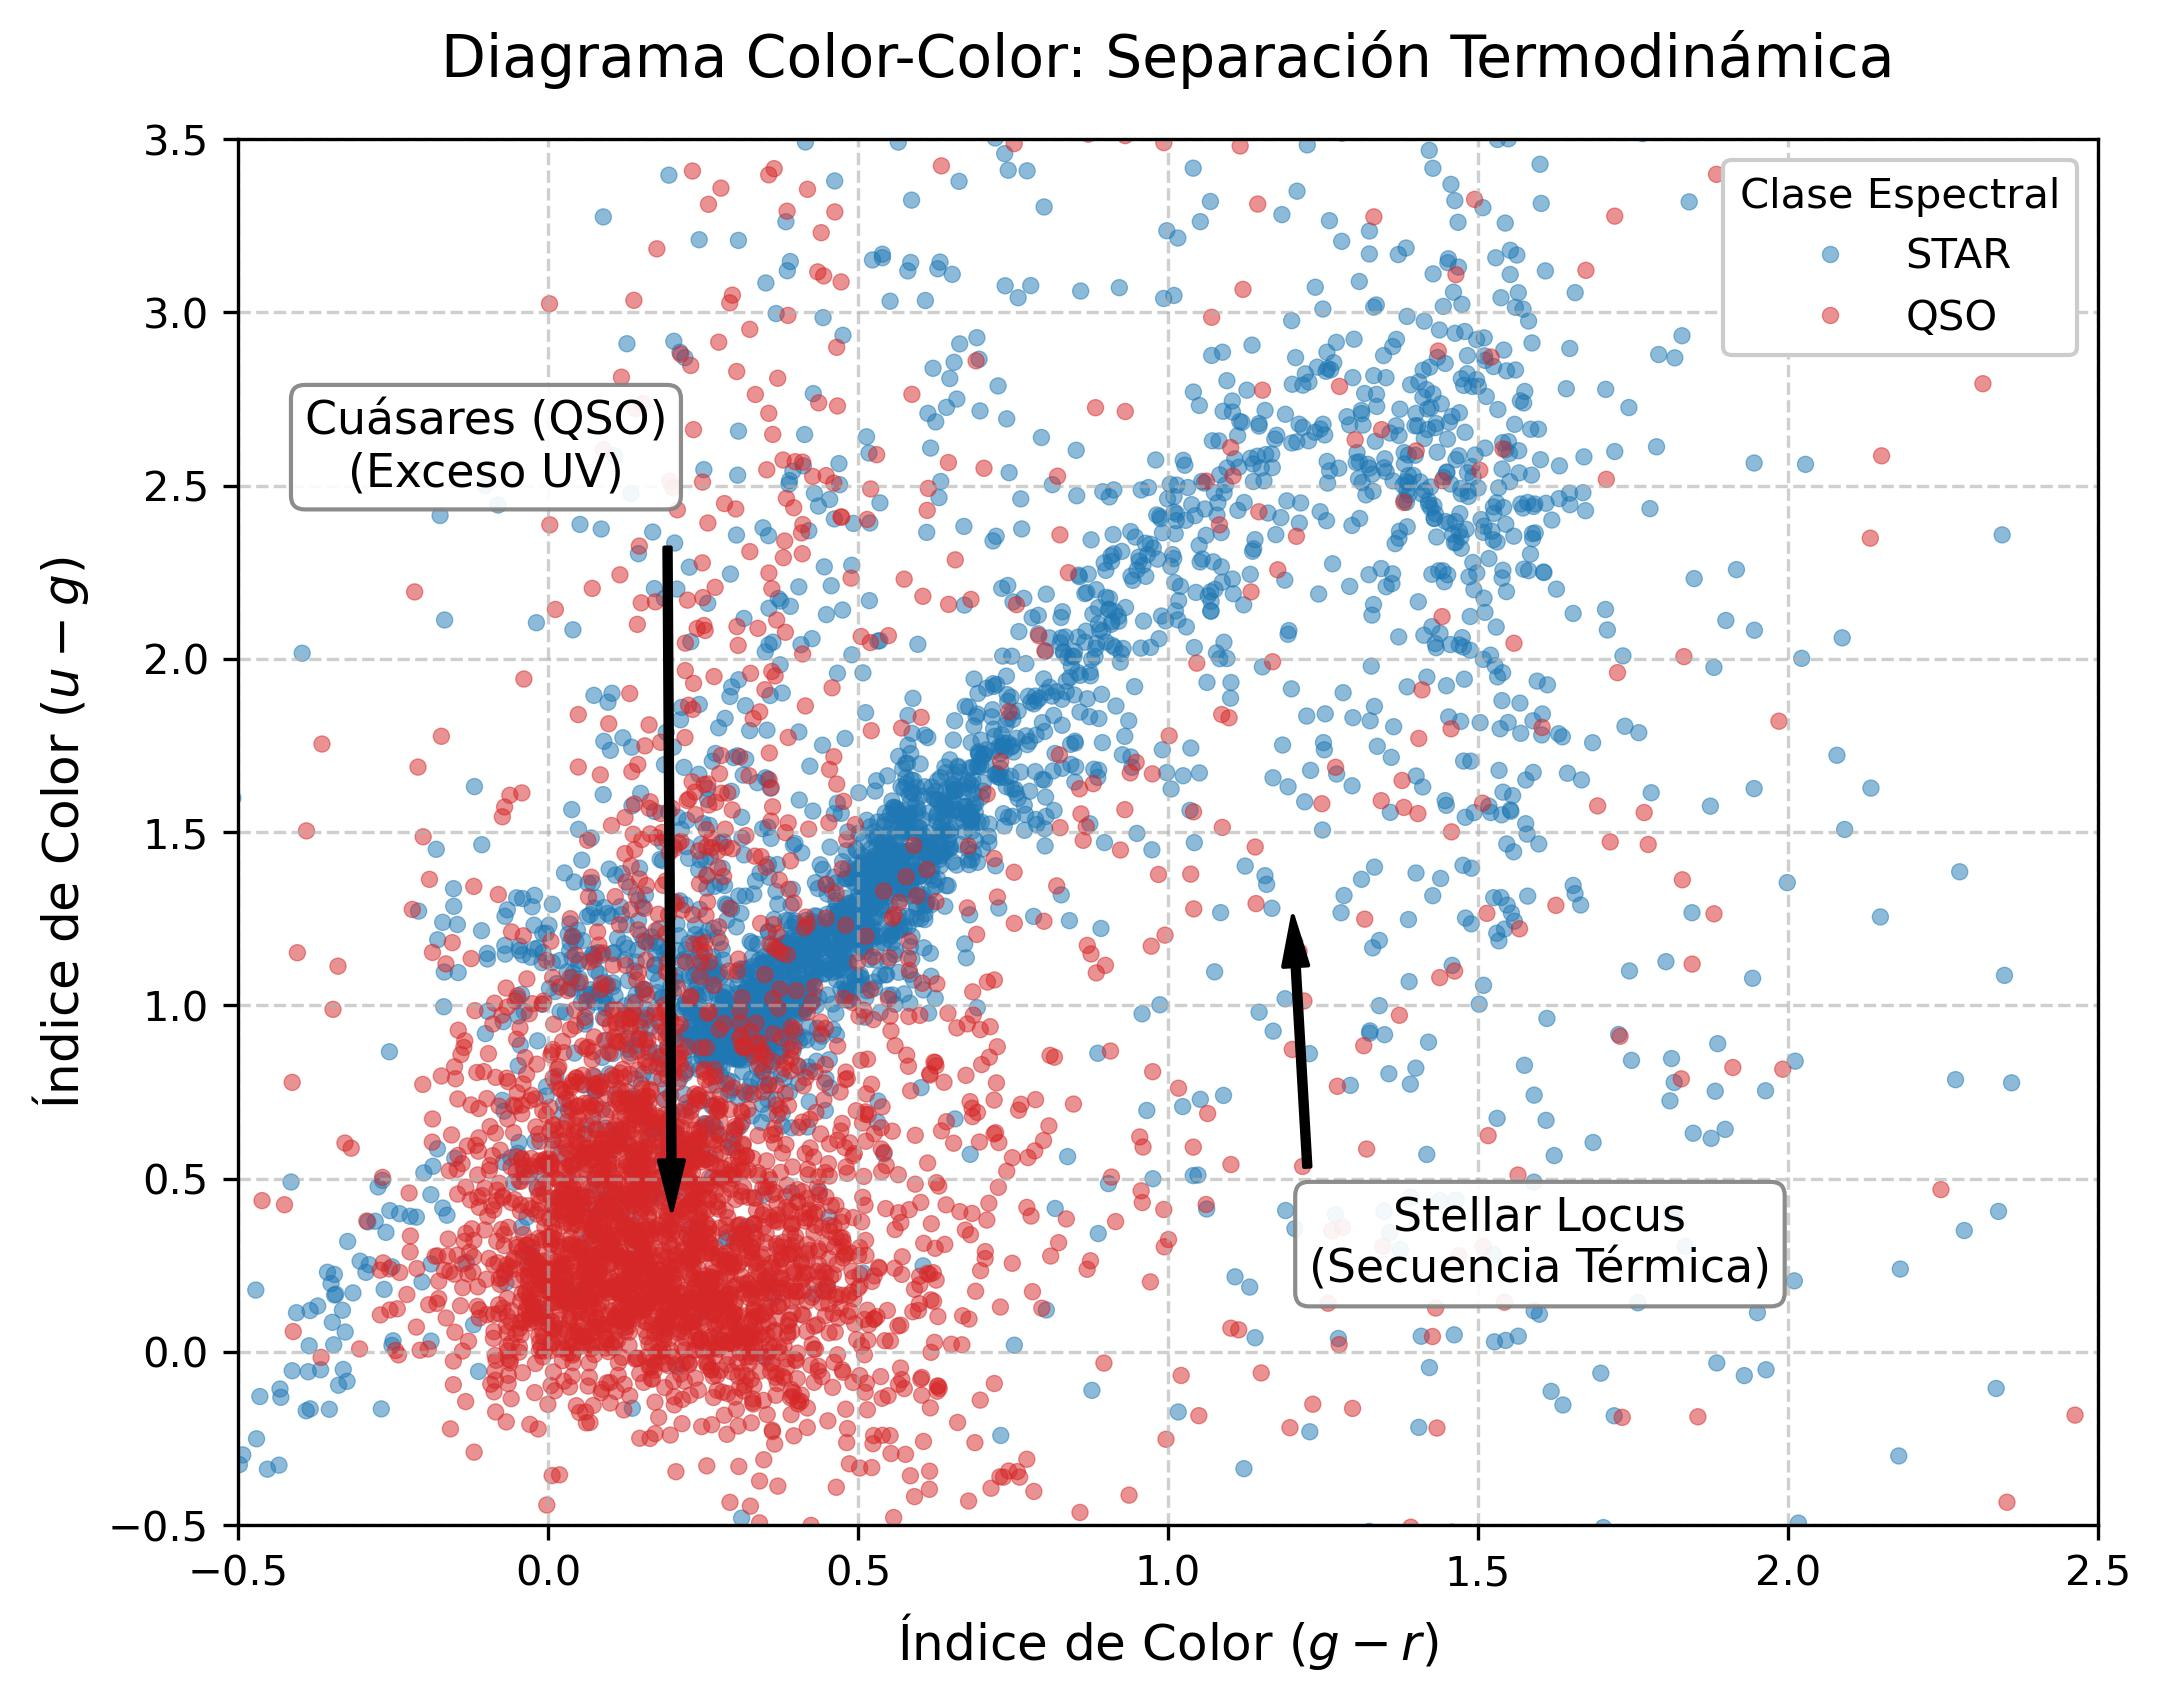
\includegraphics[width=0.8\textwidth]{stellar_locus_quasars.jpg} 
    \caption{Diagrama color-color ($u-g$ frente a $g-r$). Se aprecia claramente el \textit{Stellar Locus} formando una secuencia principal térmica, mientras que los cuásares (QSO) se aíslan en la región inferior izquierda debido a su fuerte exceso de emisión en la banda azul/UV.}
    \label{fig:stellar_locus}
\end{figure}

Un aspecto topológico crucial que revela este diagrama ---y que resulta fundamental para interpretar el rendimiento de los algoritmos analizados posteriormente--- es la aparente paradoja visual de observar únicamente dos agrupaciones principales (\textit{nubes} o \textit{locus}) a pesar de contar con tres clases taxonómicas distintas. La explicación a este fenómeno geométrico radica estrictamente en los mecanismos físicos de emisión de luz:

\begin{itemize}
    \item \textbf{Degeneración Térmica (Estrellas y Galaxias):} Las estrellas y las galaxias comparten el mismo espacio de color termodinámico. Dado que una galaxia es, en esencia, un sistema gravitacional compuesto por miles de millones de estrellas, el flujo luminoso integrado que captura el fotómetro es fundamentalmente la superposición de la emisión térmica de dicha población estelar. Por consiguiente, la inmensa mayoría de las galaxias se proyectan estadísticamente justo debajo de la secuencia principal estelar (el \textit{Stellar Locus}).
    \item \textbf{Emisión No Térmica (Cuásares):} Por el contrario, los cuásares (QSO) forman la segunda agrupación espacial aislada. Su elevada luminosidad no proviene de procesos de fusión nuclear térmica estelar, sino de la radiación originada en el disco de acreción de un agujero negro supermasivo devorando materia. Este mecanismo físico extremo produce un marcado ``exceso ultravioleta'' que desplaza drásticamente sus índices de color, separándolos visual y estadísticamente de la secuencia estelar.
\end{itemize}

Esta degeneración poblacional demuestra que separar cuásares del resto de objetos es un problema de aislamiento de emisiones anómalas, mientras que discriminar entre estrellas y galaxias requerirá que los algoritmos de Machine Learning encuentren fronteras de decisión extremadamente finas dentro del mismo espacio de color térmico.

\subsection{Estandarización de Variables}
Muchos algoritmos de aprendizaje automático, especialmente aquellos basados en distancias (K-Means, SVM) o gradientes, son sensibles a la escala de las variables de entrada. Aunque los índices de color tienen rangos similares, pequeñas variaciones de escala pueden sesgar la función de coste. Por este motivo, se ha procedido a estandarizar todas las características de entrada, transformando las distribuciones originales de modo que cada variable presente una media aritmética nula ($\mu = 0$) y una desviación típica unitaria ($\sigma = 1$).

\subsection{Partición Estratificada de Datos}
Finalmente, para evaluar la capacidad de generalización de los modelos, se dividió el conjunto de datos en dos subconjuntos disjuntos:
\begin{itemize}
    \item \textbf{Conjunto de Entrenamiento (Train):} 70\% de los datos, utilizado exclusivamente para el ajuste de los parámetros del modelo y la aplicación de técnicas de remuestreo.
    \item \textbf{Conjunto de Prueba (Test):} 30\% de los datos, reservado estrictamente para la evaluación final y validación de métricas.
\end{itemize}

Dado el desbalanceo intrínseco de clases (Fig. \ref{fig:distribucion}), se utilizó un muestreo \textbf{Estratificado}. Este método analítico asegura que la proporción exacta de Galaxias, Estrellas y Cuásares se mantenga idéntica en ambos subconjuntos, evitando que el conjunto de prueba carezca de suficientes ejemplos de las clases minoritarias para realizar una evaluación estadísticamente significativa. A nivel computacional, esta partición rigurosa se implementó utilizando la función \texttt{train\_test\_split} de la librería \textit{Scikit-Learn} para Python \citep{scikit-learn}.

%---------------------------------------------------------------------
% CAPÍTULO 4
\chapter{Desarrollo Experimental y Análisis de Resultados}
\label{chap:resultados}
%---------------------------------------------------------------------

En este capítulo se presenta la evaluación sistemática de los modelos propuestos. A nivel computacional, todos los experimentos, modelados y visualizaciones de este trabajo han sido desarrollados utilizando el lenguaje de programación Python. Para ello, se ha hecho uso de librerías estándar en el ámbito de la ciencia de datos, tales como \textit{Scikit-Learn} \citep{scikit-learn} para la implementación algorítmica, \textit{Imbalanced-Learn} para las técnicas de remuestreo, así como \textit{Pandas}, \textit{Matplotlib} y \textit{Seaborn} para el manejo estructurado y la visualización de los datos. El código desarrollado para este trabajo está disponible para su consulta en el siguiente repositorio de Google Drive: \href{https://drive.google.com/drive/folders/1zoQUG6qrf28nxJ_4eYyU2Y-u36aw-Naq?usp=drive_link}{Repositorio de Código del TFG}.

La experimentación se ha dividido en cuatro fases lógicas: configuración experimental, establecimiento de una línea base supervisada, investigación de las limitaciones no supervisadas y, finalmente, la optimización mediante técnicas de remuestreo.

\section{Configuración Experimental}

Antes de evaluar los modelos en el conjunto de prueba (\textit{Test}), es necesario definir la metodología de ajuste de sus parámetros internos. Para encontrar la configuración ideal de cada modelo sin incurrir en un sesgo de evaluación o sobreajuste (\textit{overfitting}), se utilizó la técnica de Búsqueda en Cuadrícula (\textit{Grid Search}) combinada con Validación Cruzada de $K$ pliegues (\textit{K-Fold Cross-Validation}). 

Esta técnica consiste en dividir el conjunto de entrenamiento iterativamente en $K$ subconjuntos disjuntos (en nuestro caso, $K=5$). El algoritmo se entrena en 4 de esos pliegues y se valida en el pliegue restante, repitiendo el proceso 5 veces rotando el pliegue de validación. Finalmente, se promedia el rendimiento para obtener una estimación robusta de la capacidad de generalización del modelo con esos parámetros específicos.

La Tabla \ref{tab:hiperparametros} detalla la configuración óptima encontrada para cada algoritmo. El criterio utilizado para seleccionar estos hiperparámetros como ``óptimos'' fue la maximización estricta de la métrica \textbf{F1-Macro} promediada en los pliegues de validación. Se priorizó esta métrica sobre la exactitud global (\textit{Accuracy}) para garantizar un rendimiento equilibrado en todas las clases, penalizando los modelos que ignorasen a la clase minoritaria. Además, se utilizó la semilla aleatoria \texttt{random\_state=42} para asegurar el determinismo y la reproducibilidad total en las ejecuciones.

\begin{table}[h!]
\centering
\renewcommand{\arraystretch}{1.3} % Aumenta el espacio entre filas (más volumen)
\begin{tabular}{|l|l|p{6cm}|}
\hline
\textbf{Modelo} & \textbf{Hiperparámetro} & \textbf{Valor Seleccionado} \\ \hline
\multirow{4}{*}{Random Forest} 
 & N.º Árboles (\textit{n\_estimators}) & 100 \\ \cline{2-3} 
 & Profundidad Máx. & None (Expansión completa) \\ \cline{2-3} 
 & Criterio de División & Gini \\ \cline{2-3} 
 & Mín. muestras por hoja & 1 \\ \hline
\multirow{3}{*}{SVM} 
 & Kernel & RBF (Radial Basis Function) \\ \cline{2-3} 
 & Regularización ($C$) & 10.0 \\ \cline{2-3} 
 & Gamma & 'scale' \\ \hline
\multirow{3}{*}{K-Means} 
 & N.º Clusters ($K$) & 3 (Fijado por clases físicas) \\ \cline{2-3} 
 & Inicialización & k-means++ \\ \cline{2-3} 
 & Máx. Iteraciones & 300 \\ \hline
\end{tabular}
\caption{Resumen de la configuración de hiperparámetros óptimos. Estos valores se obtuvieron maximizando explícitamente la métrica F1-Macro durante la validación cruzada.}
\label{tab:hiperparametros}
\end{table}

\section{Fase 1: Línea Base Supervisada (RF vs SVM)}

El primer experimento consistió en evaluar el rendimiento de los modelos de clasificación supervisada utilizando las características de color estandarizadas sin aplicar técnicas de balanceo adicionales. El objetivo era establecer una referencia de rendimiento (\textit{baseline}) con la que comparar los modelos tras aplicar técnicas de remuestreo y los modelos de clasificación no supervisados.

\subsection{Comparativa de Métricas}
Ambos modelos mostraron un alto desempeño global, superando el 96\% de exactitud. Sin embargo, al desglosar las métricas, se observan diferencias notables en la capacidad de generalización.

Como muestra la Tabla \ref{tab:comparativa_fase1}, Random Forest obtiene una ventaja competitiva de aproximadamente un $1.7\%$ en exactitud respecto al SVM. Físicamente, esto sugiere que las fronteras de decisión óptimas en el espacio de color son ortogonales a los ejes, lo cual favorece a la estructura de partición rectangular de los árboles de decisión frente a las fronteras suaves y curvas que intenta ajustar el kernel RBF del SVM (tal y como se ilustró al explicar el funcionamiento teórico de estos algoritmos en el Capítulo 2).

\begin{table}[H]
\centering
\renewcommand{\arraystretch}{1.2}
\begin{tabular}{|l|c|c|c|c|}
\hline
\textbf{Modelo} & \textbf{Accuracy} & \textbf{Precision} & \textbf{Recall} & \textbf{F1-Score} \\ \hline
Random Forest & 97.82\% & 0.97 & 0.96 & 0.97 \\ \hline
SVM (RBF) & 96.10\% & 0.95 & 0.93 & 0.94 \\ \hline
\end{tabular}
\caption{Promedios macro de las métricas en el conjunto de prueba (Test). El promedio ``macro'' calcula la métrica para cada clase de forma independiente y luego extrae la media aritmética, otorgando el mismo peso estadístico a la clase minoritaria que a la mayoritaria. Random Forest supera a SVM en todas las categorías, destacando especialmente en el Recall, métrica que evalúa la proporción de verdaderos positivos recuperados frente al total real de observaciones de dicha clase.}
\label{tab:comparativa_fase1}
\end{table}

\subsection{Análisis Visual de Errores}

Aunque las métricas estadísticas promediadas certifican un alto rendimiento cuantitativo, estas no revelan la naturaleza espacial de las clasificaciones erróneas. Para comprender la topología del error y su correlación directa con la física subyacente de los objetos astronómicos, se procedió a visualizar la distribución de los fallos proyectada sobre el espacio de color principal ($u-g$ frente a $g-r$). Este enfoque analítico permite determinar si los modelos se equivocan de manera aleatoria a causa del ruido instrumental, o si los errores se concentran sistemáticamente en fronteras de alta ambigüedad espectral.

\begin{figure}[hbt!]
    \centering
    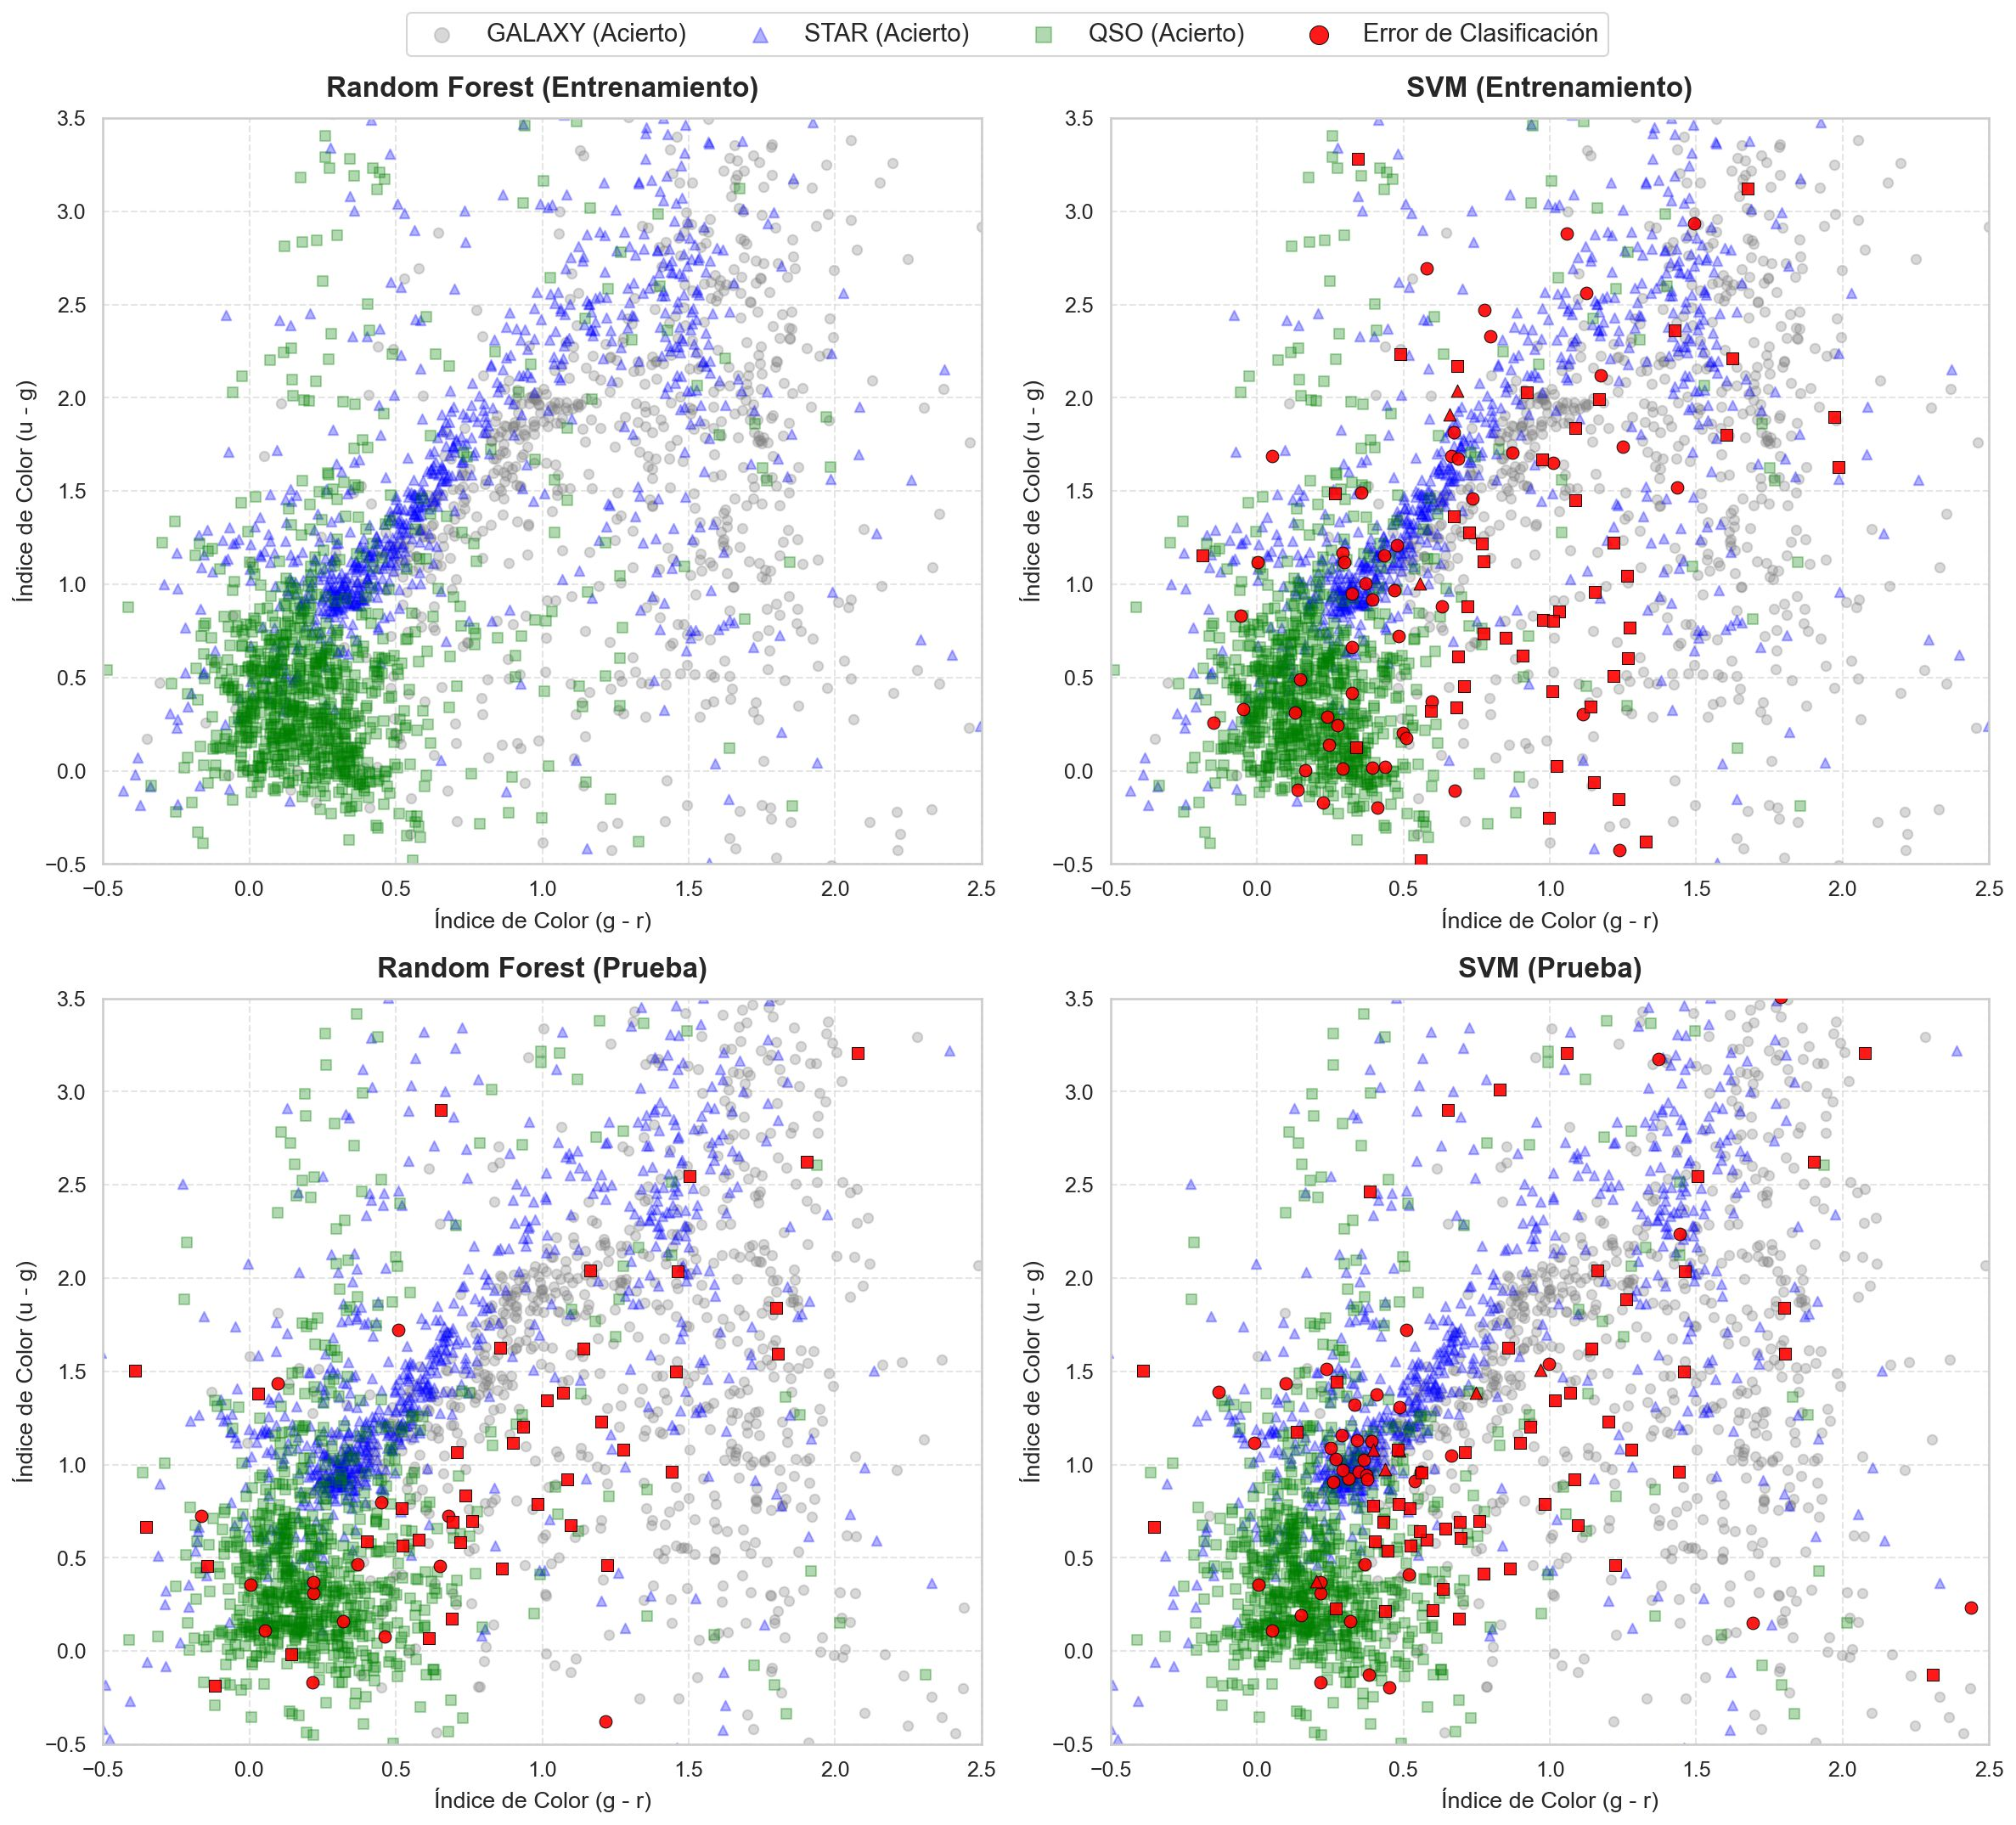
\includegraphics[width=\textwidth]{5_super_panel_errores.jpg}
    \caption{Panel comparativo de errores fotométricos ($u - g$ vs $g - r$) para los conjuntos de entrenamiento y prueba. Las clasificaciones correctas se muestran semitransparentes (Galaxias en gris, Estrellas en azul, Cuásares en verde), mientras que los fallos se superponen en rojo intenso. Se observa que el modelo SVM tiene mayor dificultad en la zona de solapamiento entre la población estelar y los cuásares, mientras que Random Forest logra aislar mejor los casos límite.}
    \label{fig:panel_errores}
\end{figure}

La Figura \ref{fig:panel_errores} revela que la mayoría de los errores se concentran en la intersección de la secuencia térmica principal con la región de exceso ultravioleta propia de los cuásares. Random Forest demostró una mayor robustez para aislar los cuásares (cuadrados verdes) de las estrellas (triángulos azules) gracias a su capacidad de crear reglas de decisión locales y ortogonales muy específicas en estas regiones de alta densidad.

\section{Fase 2: Clasificación No Supervisada}

Una de las preguntas de investigación de este trabajo planteaba si la estructura intrínseca de los datos permitía una clasificación automática sin necesidad de etiquetas (Clustering). Para ello, vamos a analizar la dimensionalidad subyacente del espacio fotométrico mediante técnicas de reducción y evaluar la viabilidad de los algoritmos de agrupamiento geométrico.

\subsection{Dimensionalidad Intrínseca (PCA)}

Primero, se aplicó un Análisis de Componentes Principales (PCA) para verificar si las clases eran separables linealmente en un espacio reducido. Para evaluar la cantidad de información retenida, se analizó el \textbf{gráfico de sedimentación} (\textit{Scree Plot}). Esta representación gráfica bidimensional ordena las componentes principales de mayor a menor según la proporción de varianza total que explican. Su propósito analítico es identificar visualmente el punto de inflexión o ``codo'' de la curva, lo que permite determinar cuántas dimensiones son estrictamente necesarias para representar la estructura subyacente de los datos sin perder información crítica.

Como se observa en la Figura \ref{fig:pca_combined}a, las dos primeras componentes solo explican el $\sim 62\%$ de la varianza, y el gráfico de sedimentación revela que se necesitan al menos 4 componentes para capturar el 90\% de la información. Esto tiene una interpretación física importante: la información espectral contenida en los 5 filtros no es redundante; cada banda aporta información única sobre la temperatura o el redshift, impidiendo una reducción simplista a 2D sin pérdida crítica de información.

Al proyectar los datos en las dos primeras componentes principales (Figura \ref{fig:pca_combined}b), se confirma visualmente el problema: las clases forman un continuo topológico (una distribución espacial conexa con alta superposición de densidades) en lugar de agrupaciones discretas y separables.

% --- FIGURA COMBINADA PCA ---
\begin{figure}[hbt!]
    \centering
    \begin{subfigure}[b]{0.48\textwidth}
        \centering
        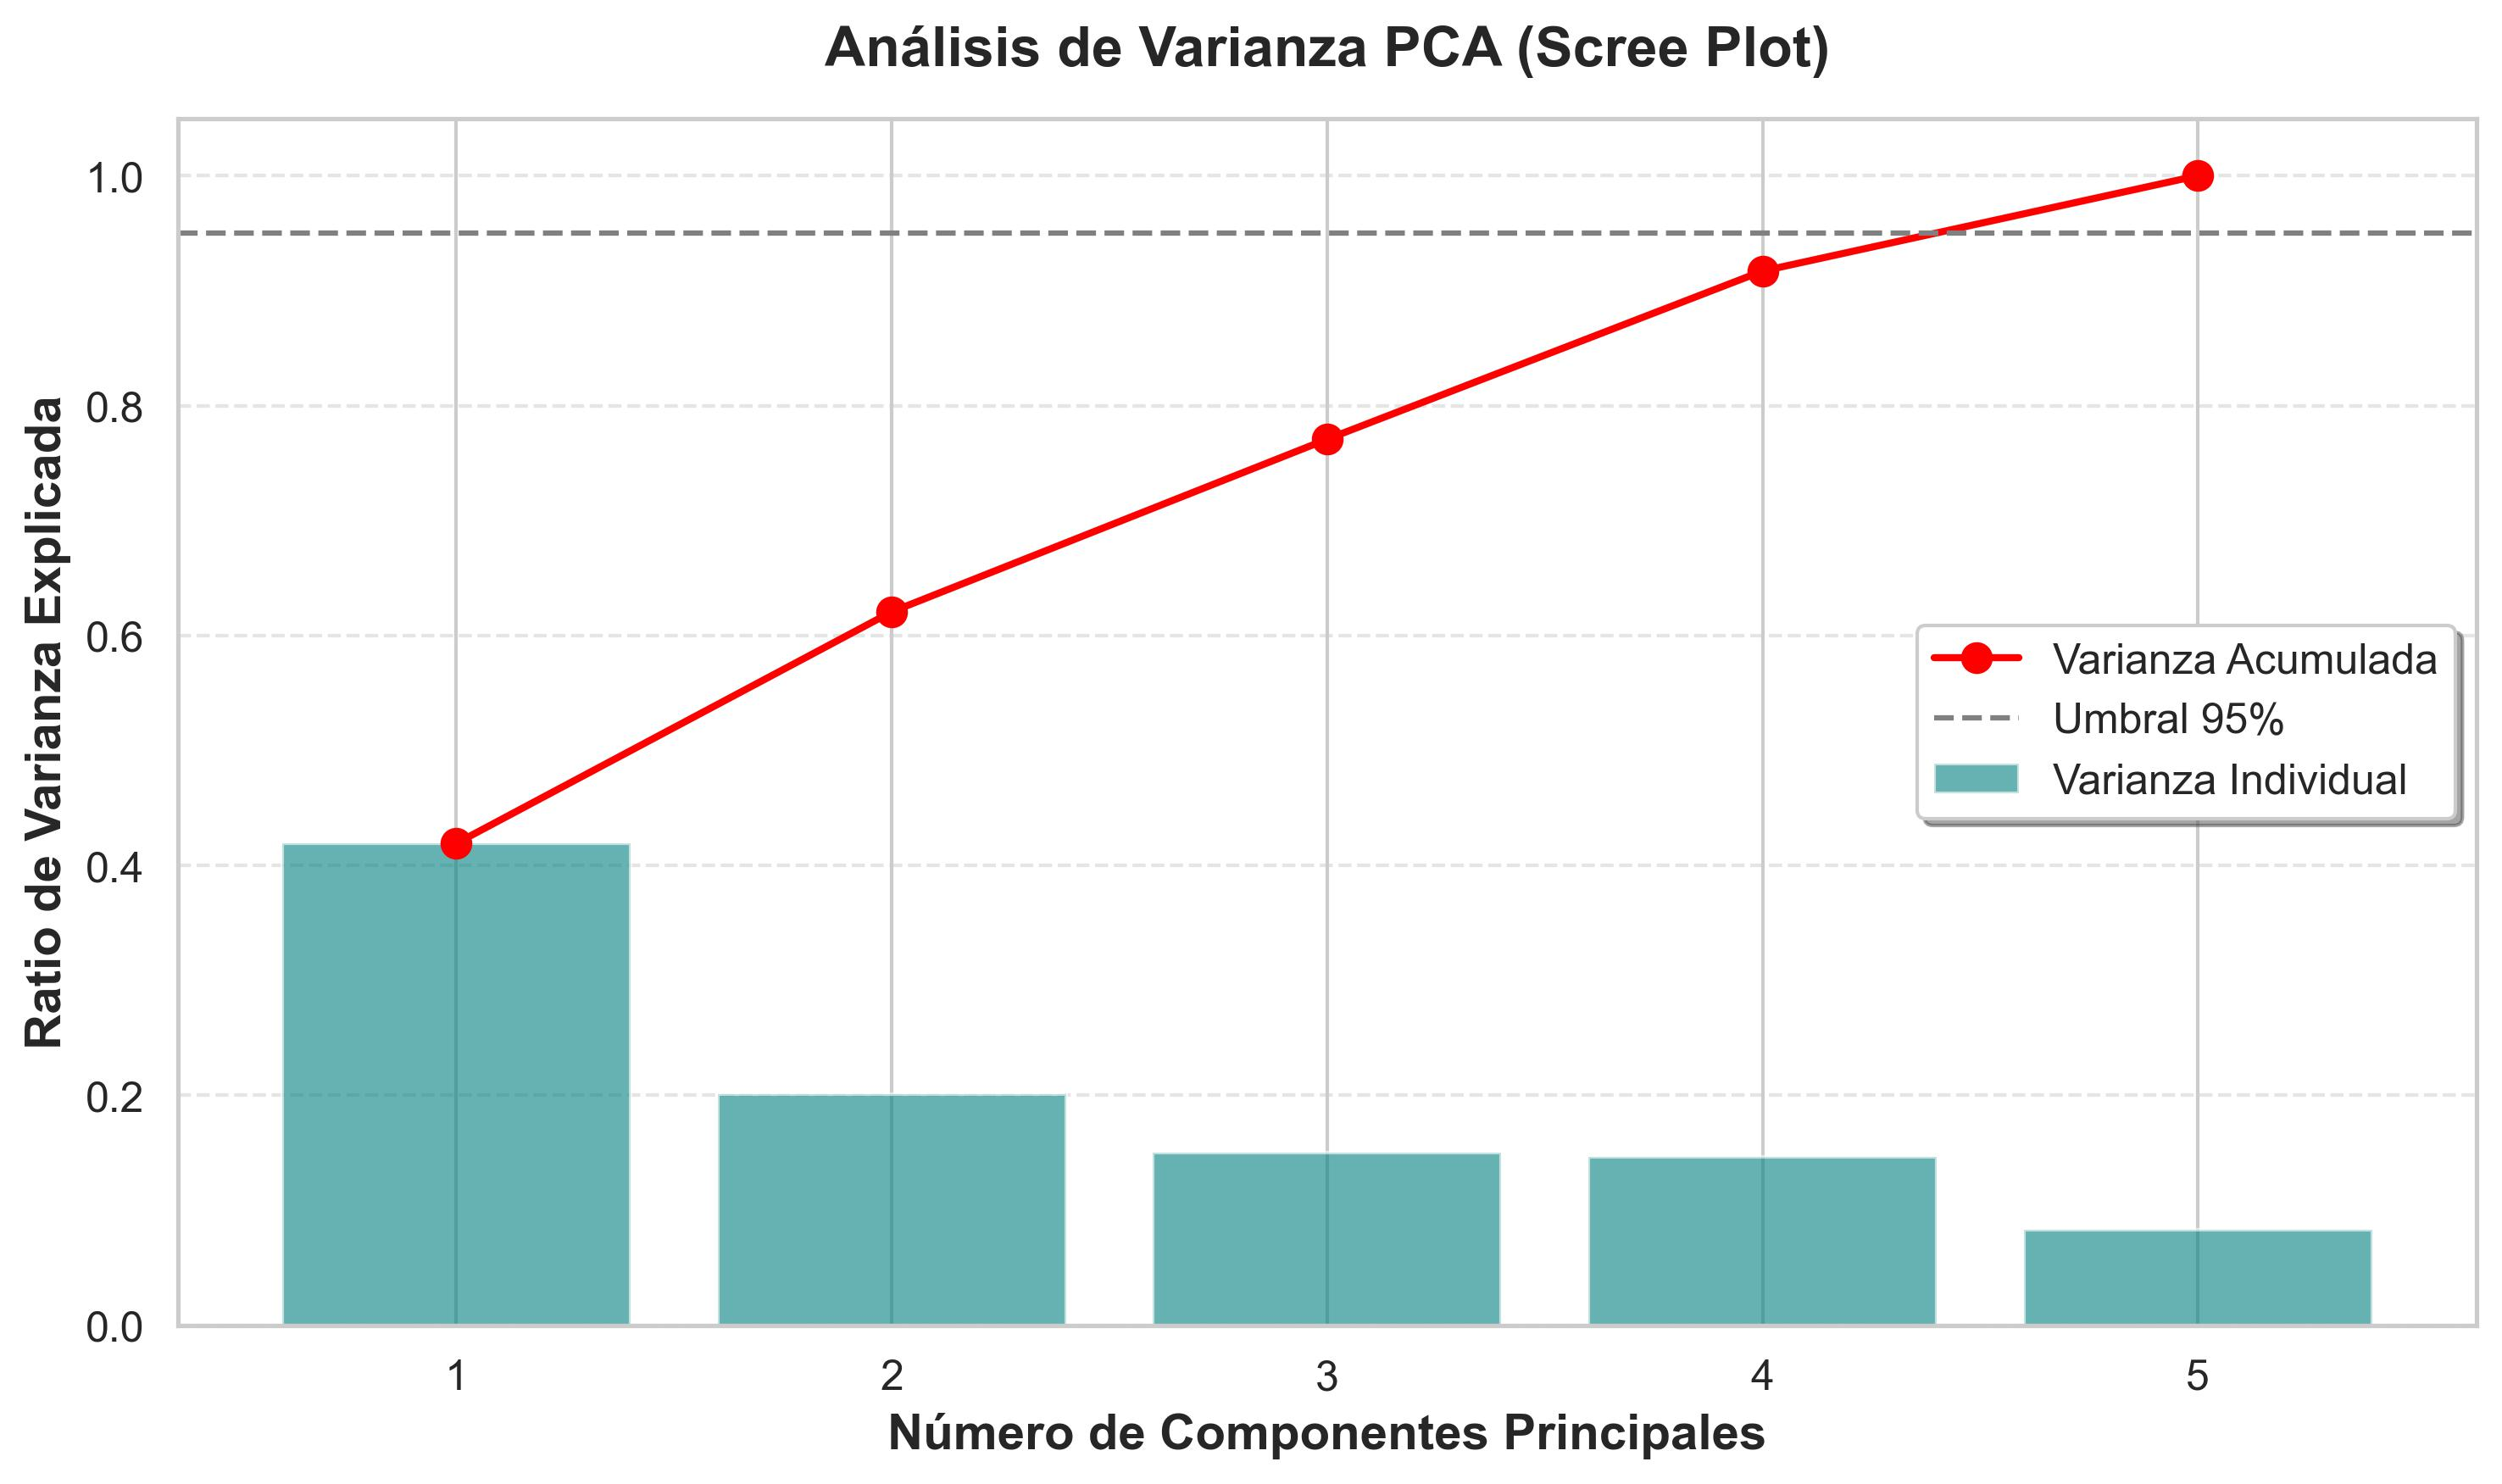
\includegraphics[width=\textwidth]{6_pca_varianza.jpg}
        \caption{Gráfico de sedimentación.}
        \label{fig:scree_plot}
    \end{subfigure}
    \hfill
    \begin{subfigure}[b]{0.48\textwidth}
        \centering
        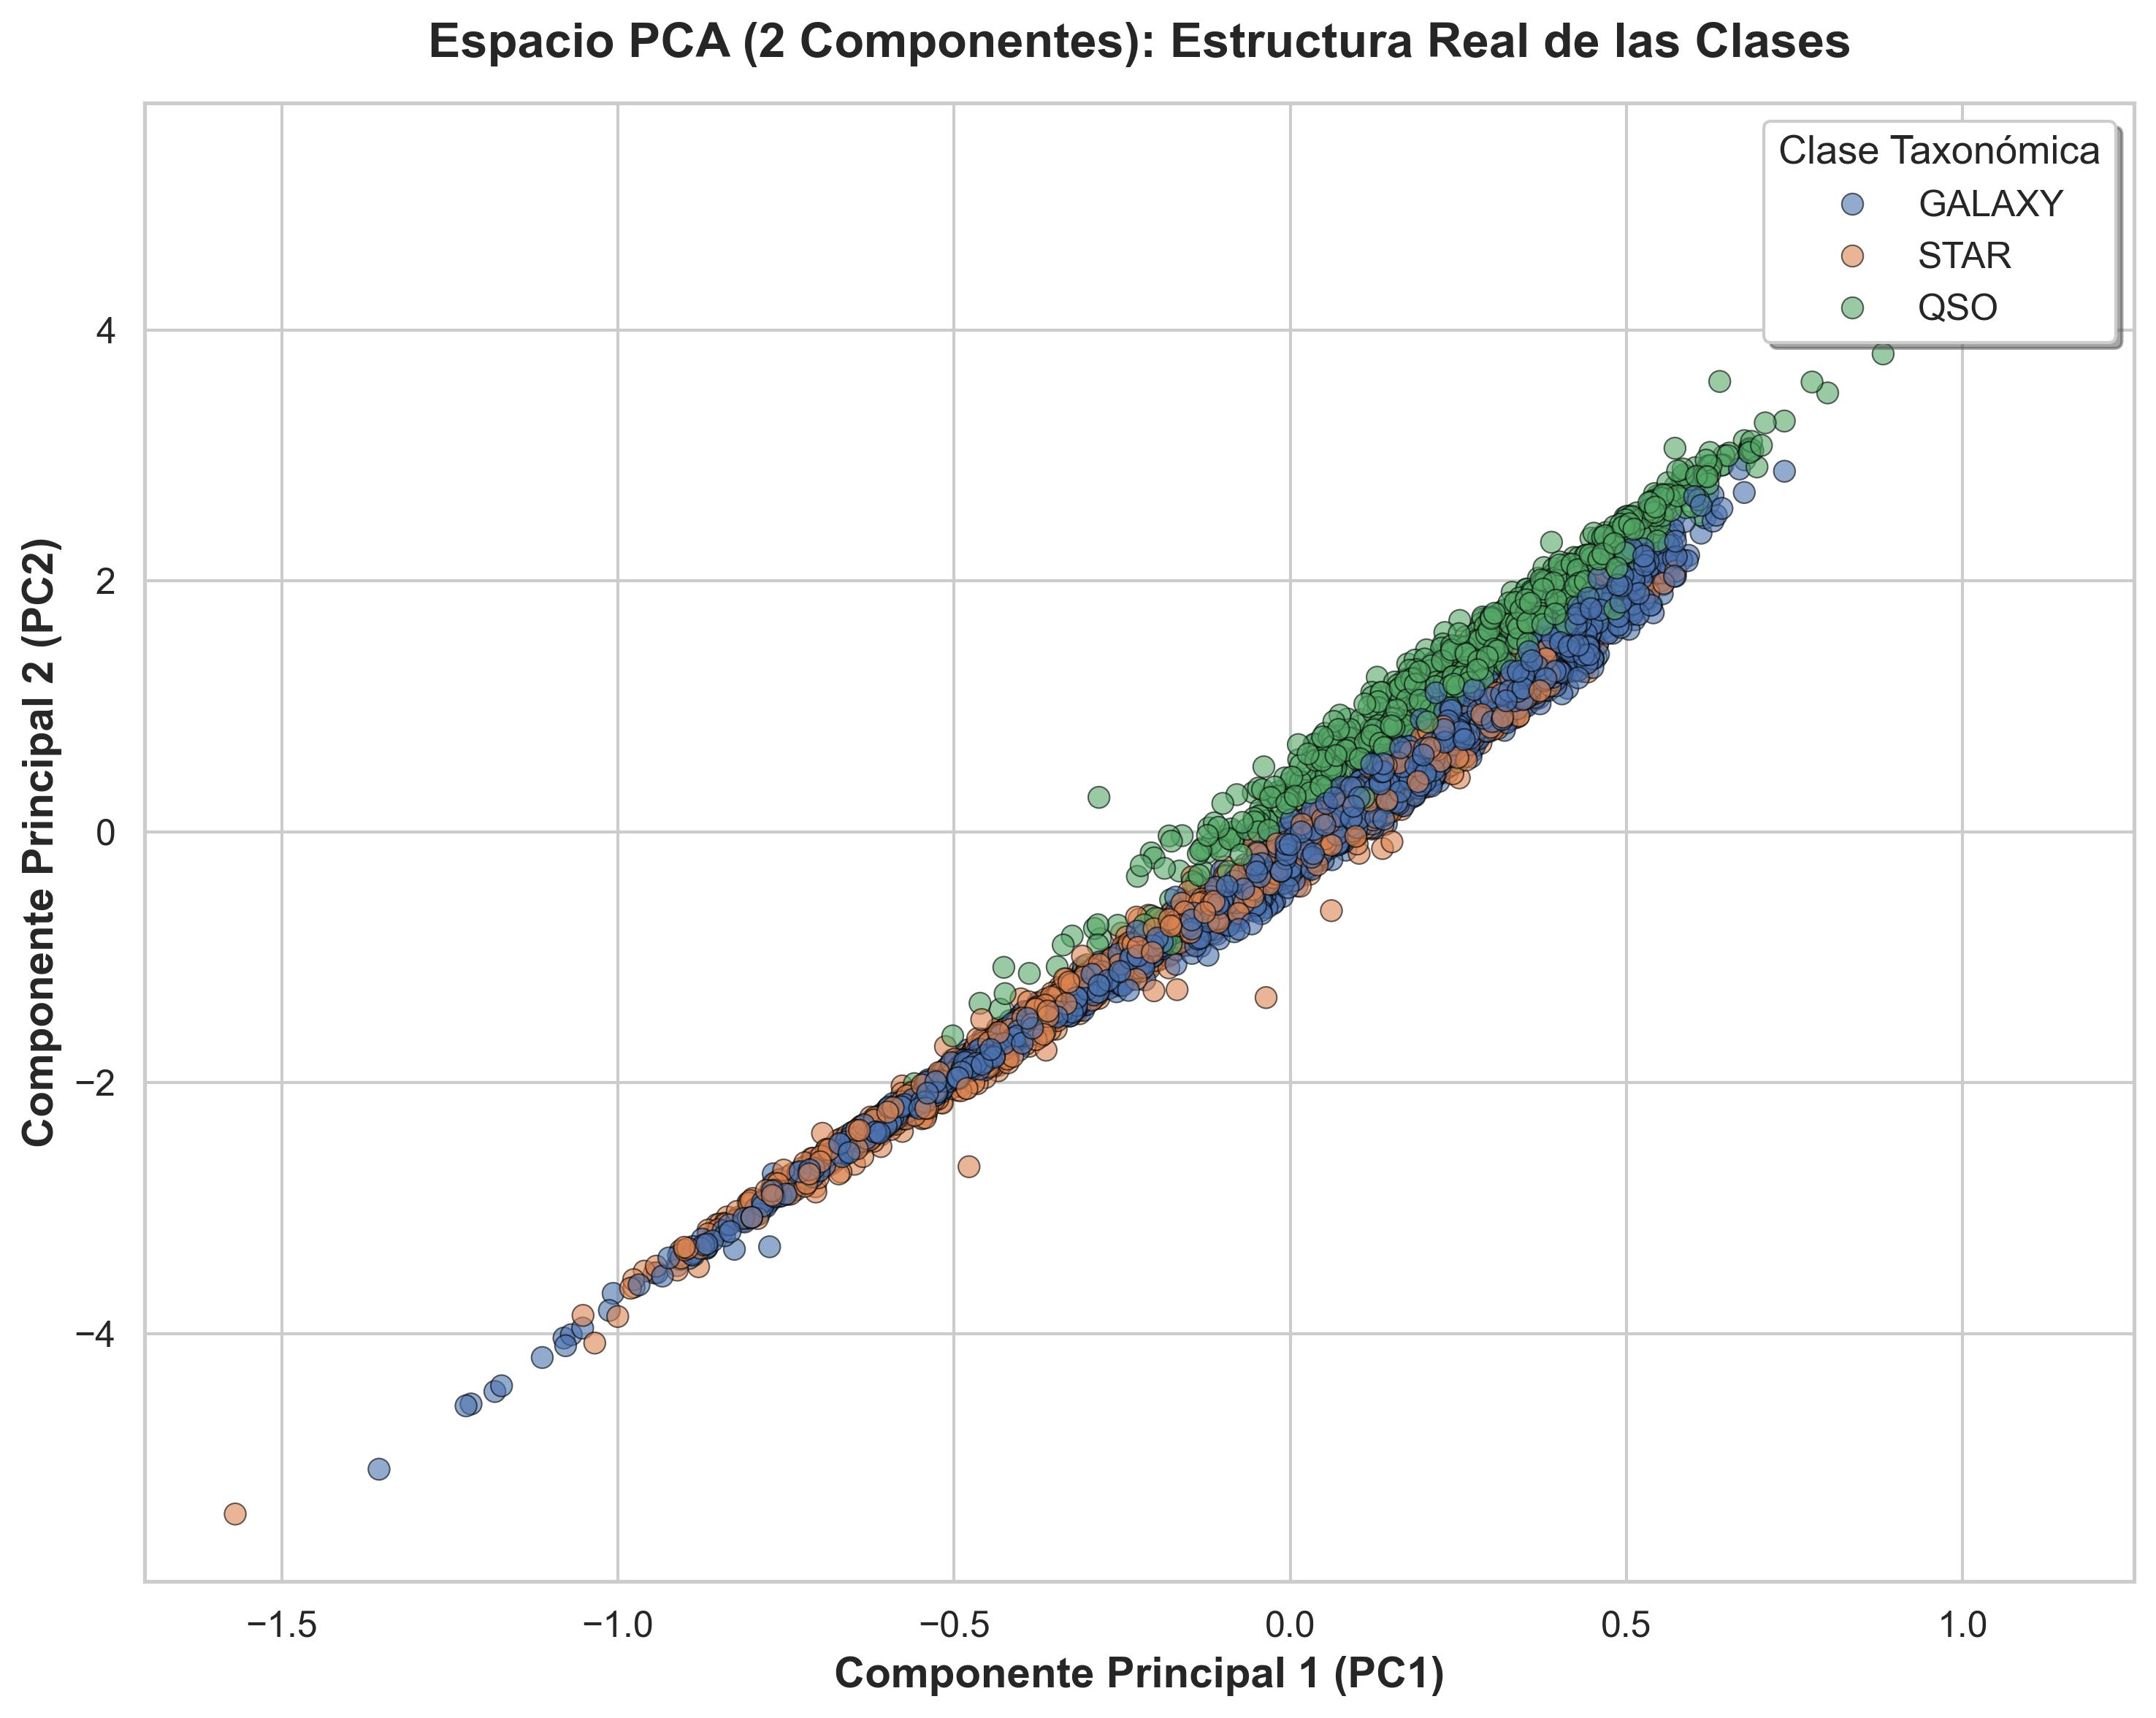
\includegraphics[width=\textwidth]{2_pca_real.jpg}
        \caption{Proyección PCA (Etiquetas Reales).}
        \label{fig:pca_real}
    \end{subfigure}
    \caption{Análisis de dimensionalidad intrínseca. (a) El gráfico de sedimentación muestra que las dos primeras componentes (62\%) son insuficientes para explicar la varianza total, indicando una estructura multidimensional compleja. (b) La proyección espacial confirma un severo solapamiento topológico entre Estrellas, Galaxias y Cuásares en el centro de la distribución.}
    \label{fig:pca_combined}
\end{figure}

\subsection{Resultados de K-Means}

Al aplicar el algoritmo K-Means configurado empíricamente con $K=3$ (correspondiente a las tres clases físicas esperadas), el rendimiento fue marcadamente insatisfactorio. Cabe aclarar metodológicamente que el modelo de agrupamiento se entrenó de forma independiente utilizando todo el espacio de características estandarizado (los índices de color fotométrico), empleando la proyección PCA de la Figura \ref{fig:pca_kmeans} de manera exclusiva como herramienta de visualización bidimensional de los grupos resultantes. 

La razón analítica de este bajo desempeño radica en la función de coste del propio algoritmo: K-Means busca minimizar la inercia (la varianza intra-cluster), lo que implícitamente asume que las agrupaciones son esféricas, compactas y de densidades uniformes. Como se evidencia en la Figura \ref{fig:pca_kmeans}, en lugar de aislar las distribuciones físicas reales, el algoritmo forzó una partición geométrica del espacio basada puramente en la proximidad euclídea (generando una teselación de Voronoi). Esto resulta en cortes artificiales que fracturan el continuo topológico del \textit{Stellar Locus}, demostrando que los modelos basados exclusivamente en métricas de distancia lineal son incapaces de capturar las complejas fronteras no convexas que separan a las clases astronómicas en un espacio puramente fotométrico.

\begin{figure}[hbt!]
    \centering
    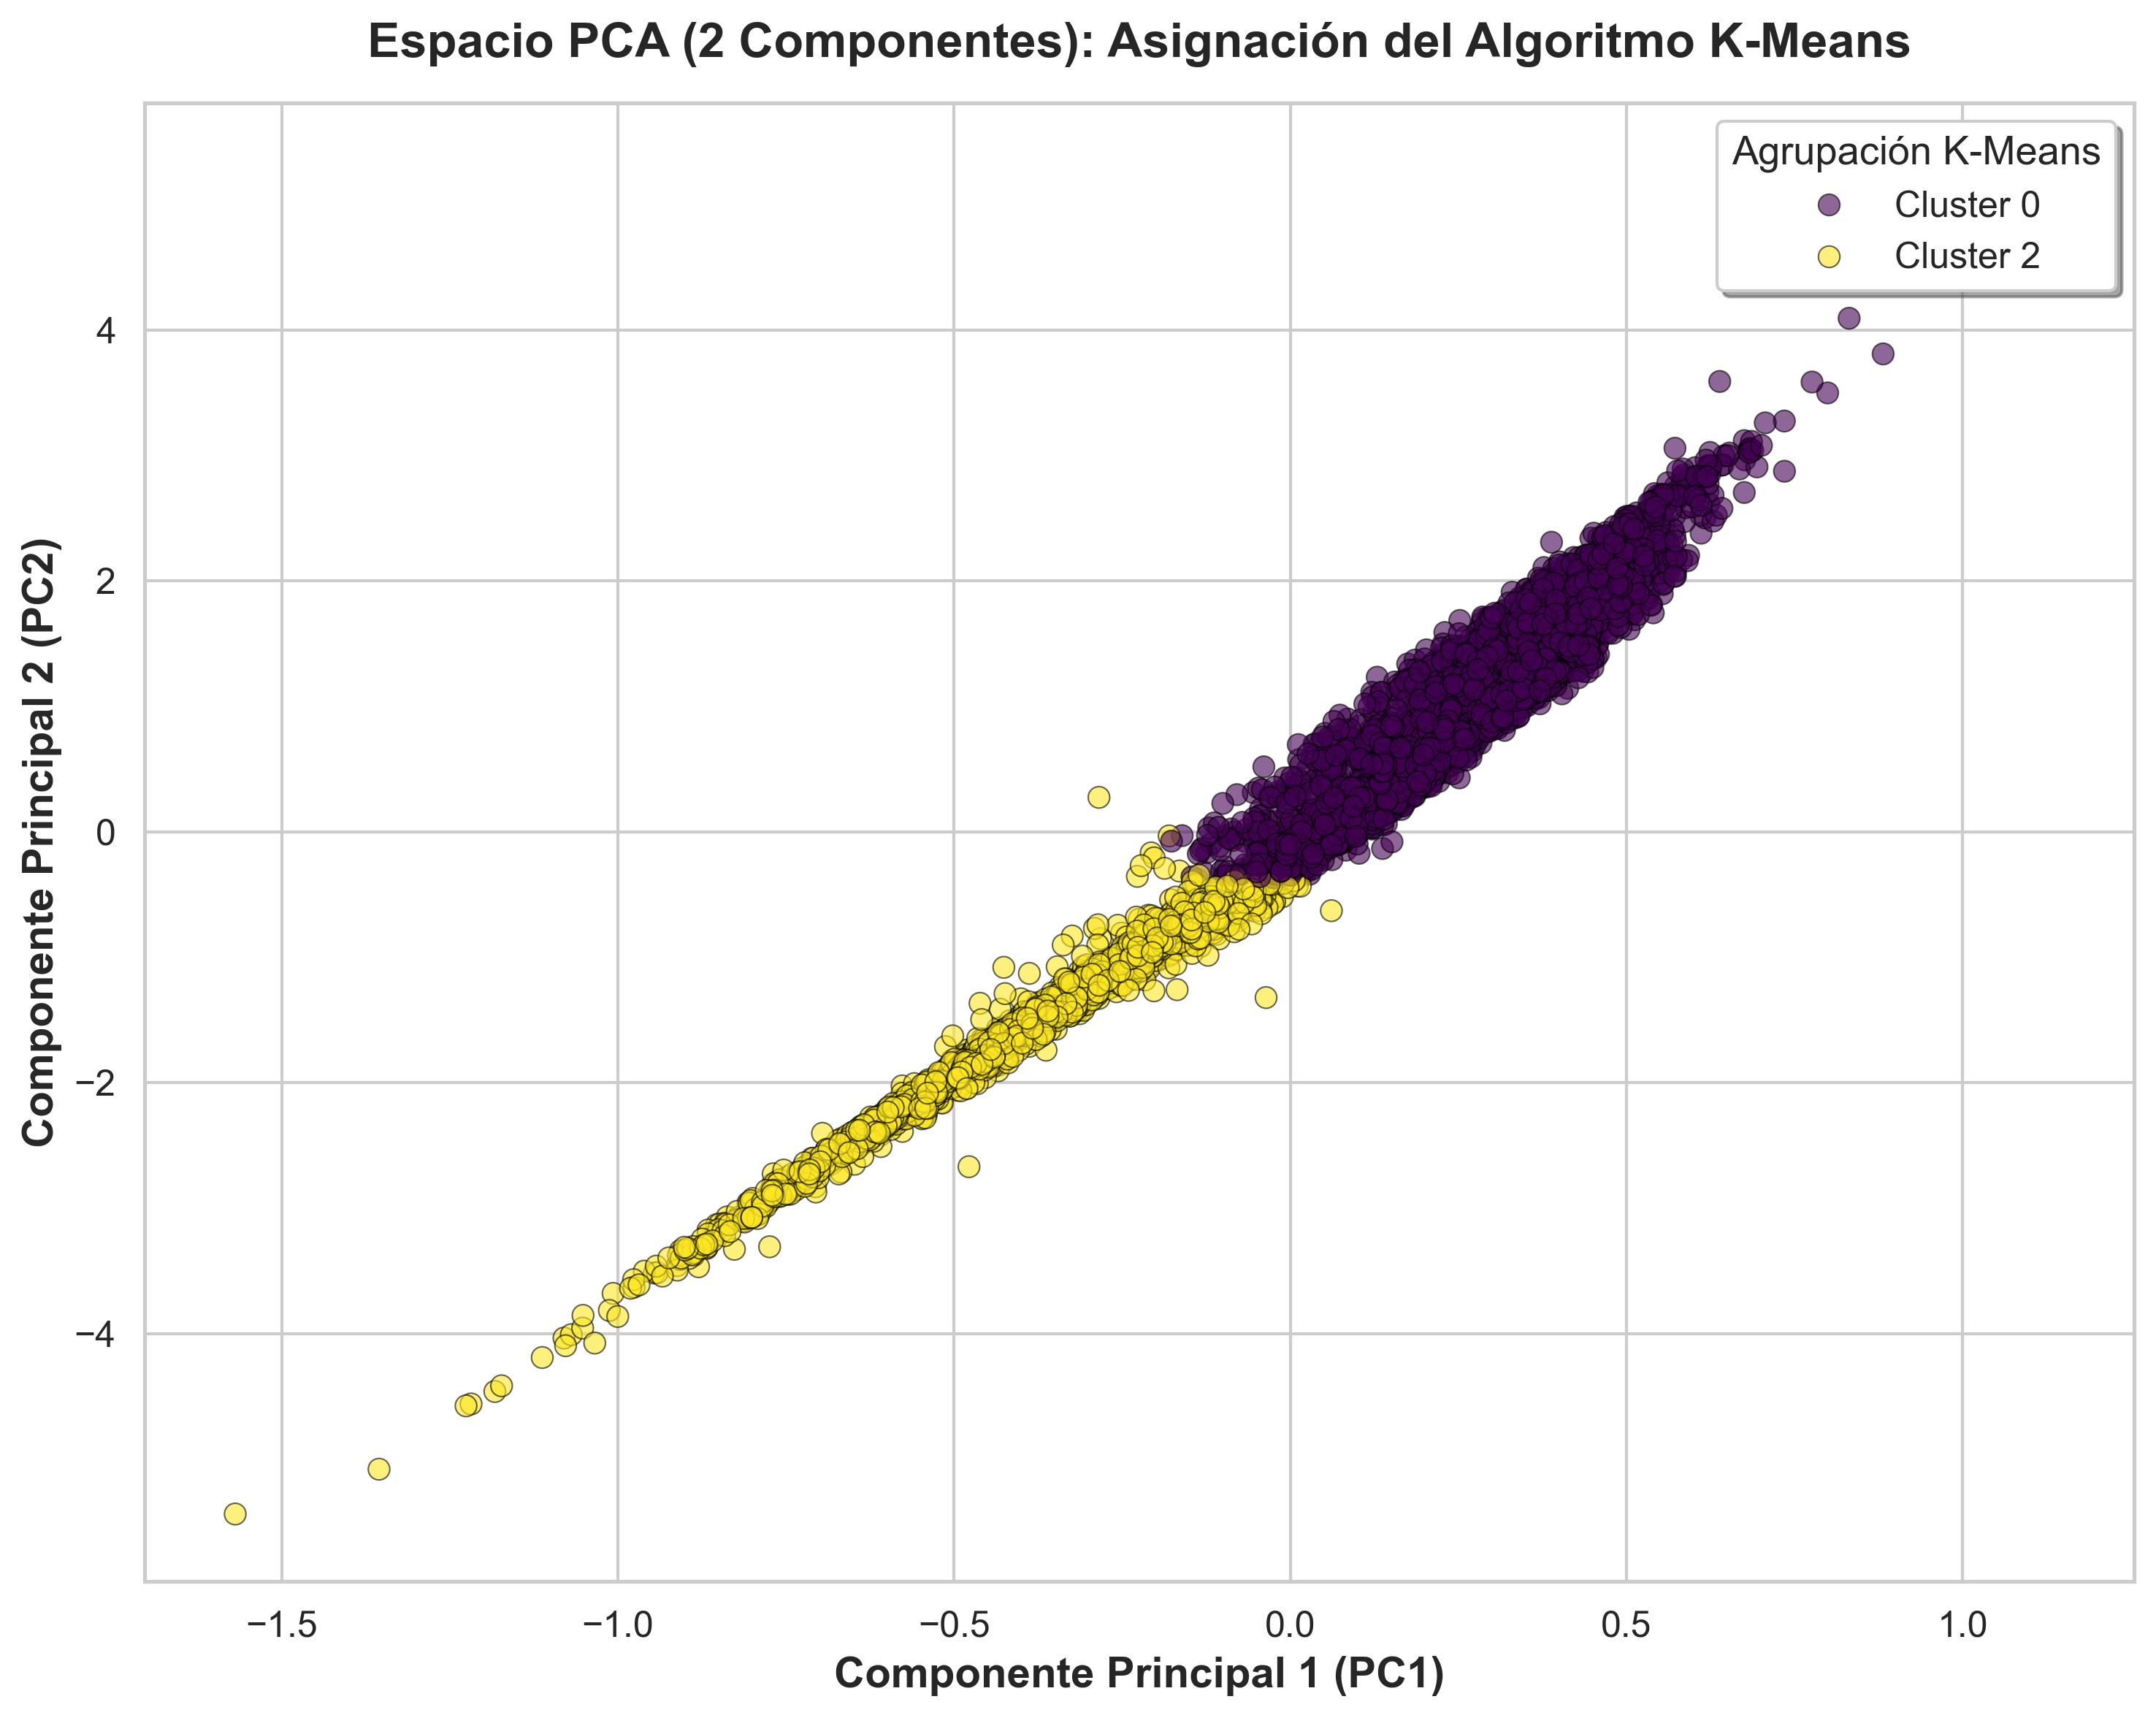
\includegraphics[width=0.65\textwidth]{3_pca_kmeans.jpg}
    \caption{Resultado de K-Means. El algoritmo divide los datos en regiones geométricas arbitrarias, siendo incapaz de seguir la densidad natural y las formas no convexas de las clases astronómicas.}
    \label{fig:pca_kmeans}
\end{figure}

\section{Fase 3: El Experimento de Control (Redshift)}

Ante el fracaso sistémico de los métodos no supervisados sobre el espacio de características original, se hizo imperativo aislar la causa raíz del problema para comprender si se trataba de una limitación intrínseca de los algoritmos de agrupamiento o de una carencia estructural en los datos de entrada. Se planteó la hipótesis de que la alta superposición observada en los diagramas de color-color es consecuencia directa de proyectar un universo inherentemente tridimensional en un plano observacional bidimensional. Es decir, se produce una profunda degeneración espacial debido a la ausencia de información de profundidad, donde objetos con naturalezas físicas radicalmente distintas (como una estrella enana cercana y un cuásar a miles de millones de años luz) pueden presentar perfiles fotométricos de color casi idénticos.

Para validar esta hipótesis, se diseñó un experimento de control empírico re-entrenando el algoritmo K-Means sobre un espacio de características ampliado que incorporaba la variable \textit{redshift} ($z$). Es fundamental destacar que el \textit{redshift} (corrimiento al rojo) no constituye una variable matemática artificial añadida para forzar el rendimiento del modelo, sino un parámetro físico riguroso derivado de mediciones espectroscópicas. En el contexto astrofísico, y en concordancia con la ley de Hubble-Lemaître \citep{hubble1929}, el \textit{redshift} actúa como un indicador directo de la distancia cosmológica y de la velocidad de recesión de los objetos extragalácticos. Al introducir esta dimensión, se restituye la topología espacial real de las fuentes.

\begin{figure}[hbt!]
    \centering
    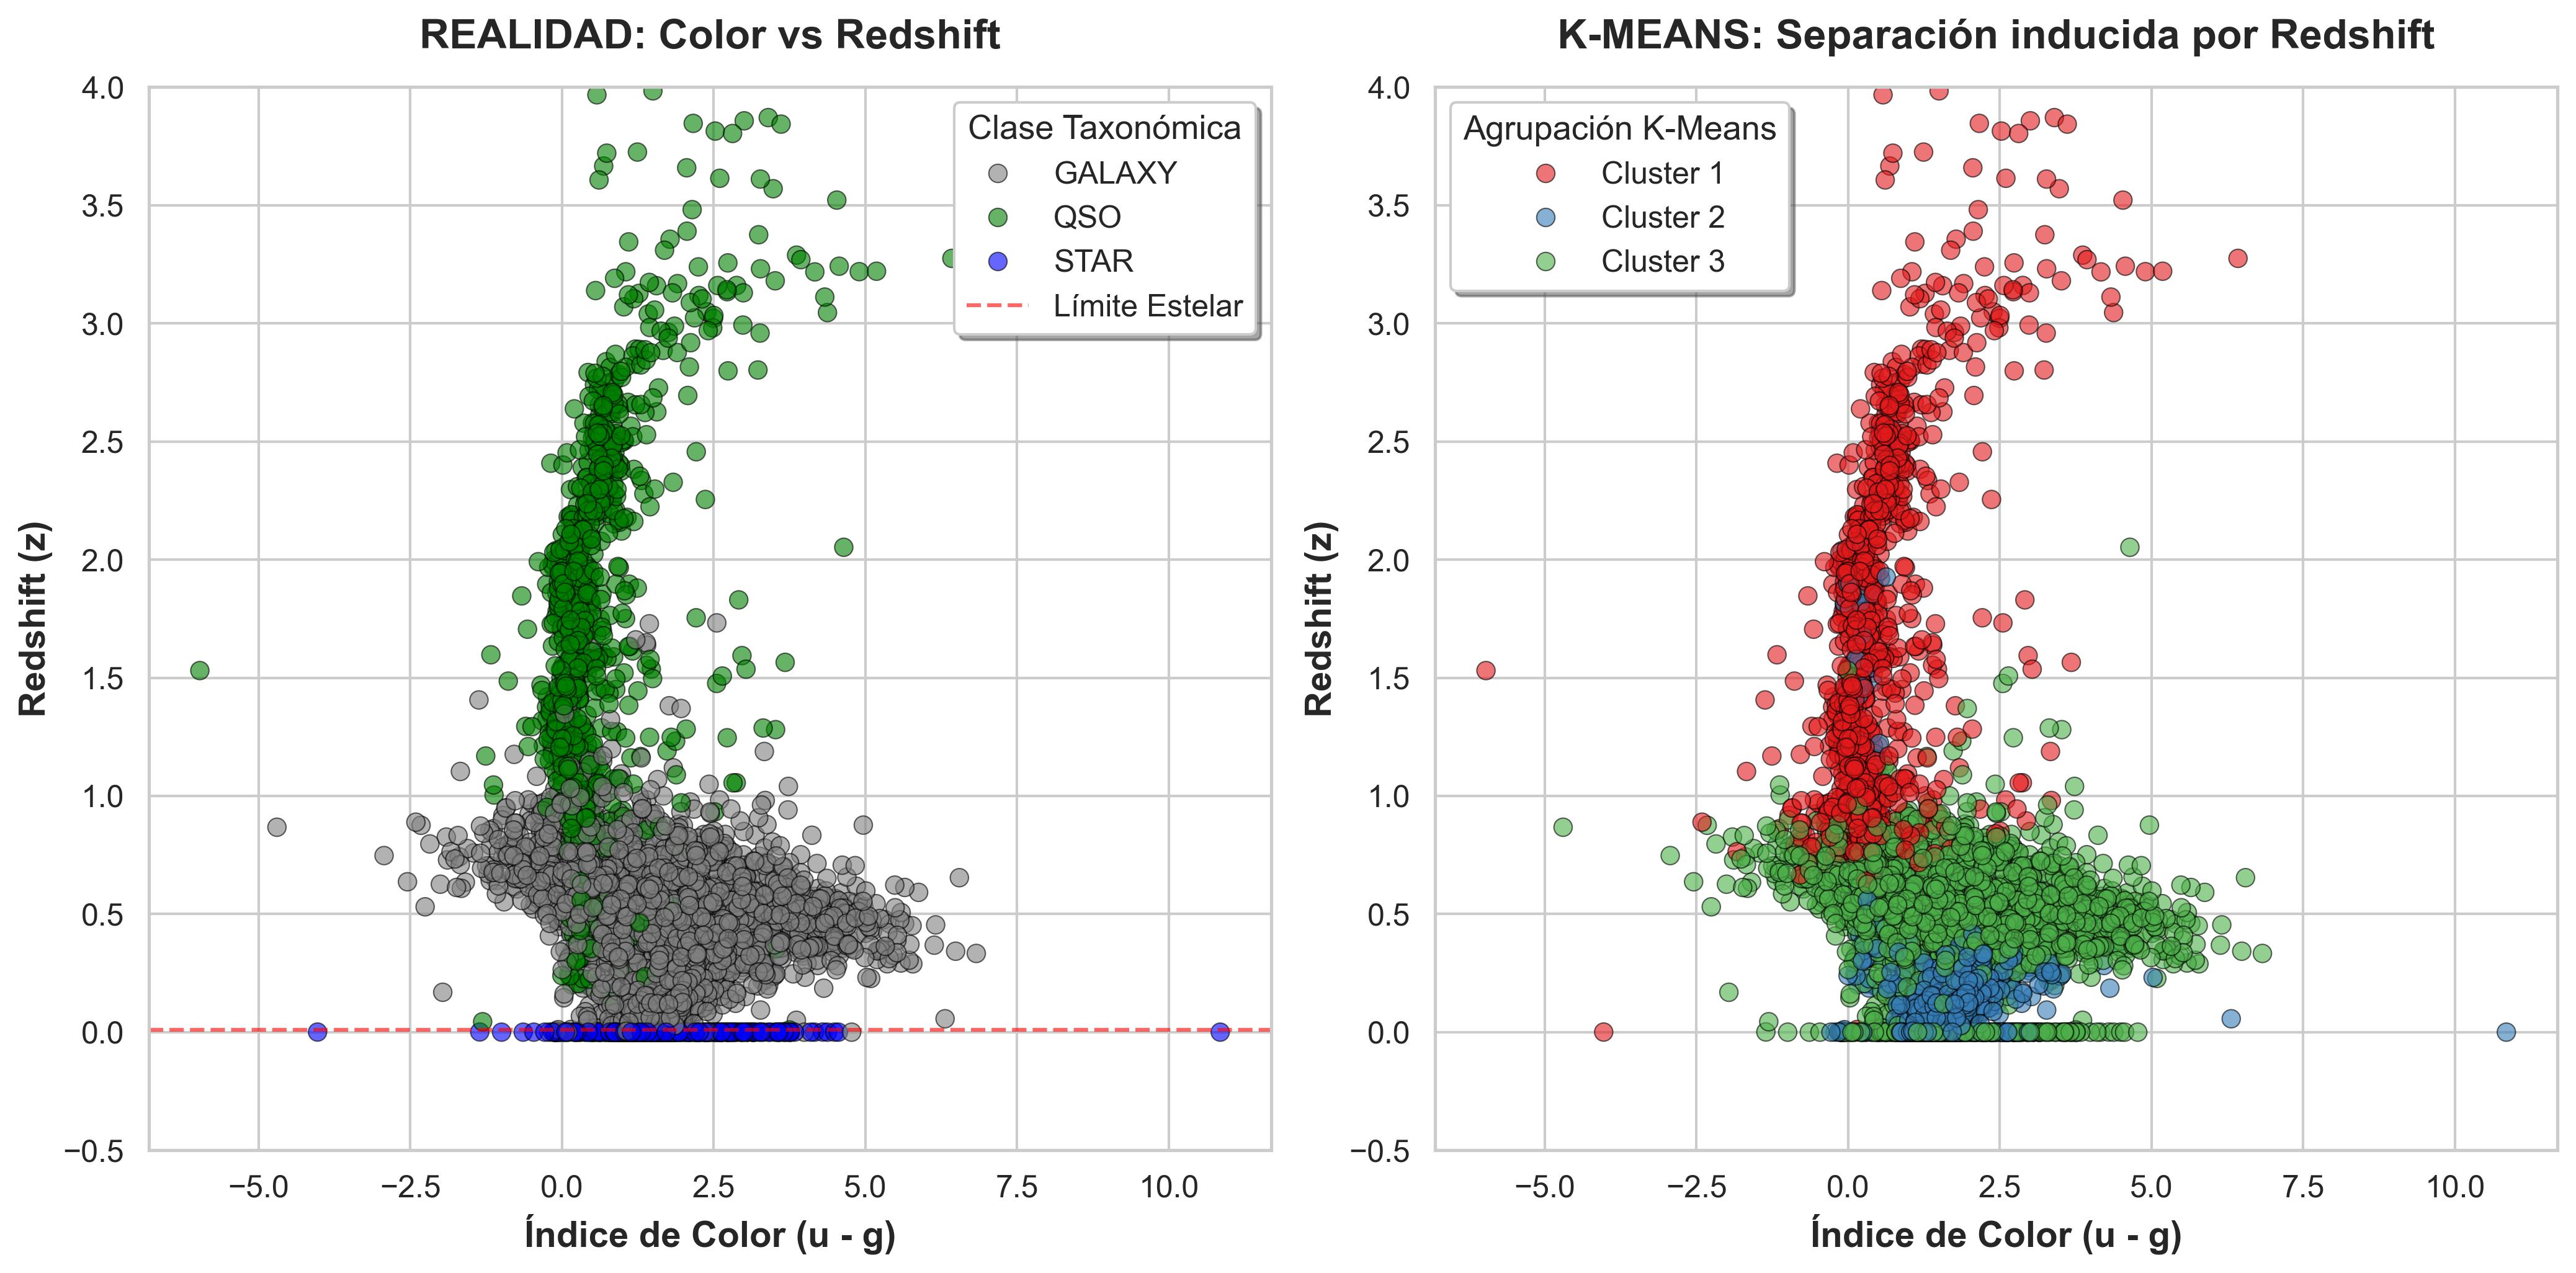
\includegraphics[width=\textwidth]{14_trampa_redshift.jpg}
    \caption{Resultados de K-Means con distintos parámetros. A la izquierda, el clustering utilizando exclusivamente características de color fotométrico, donde se observa la mezcla topológica y la incapacidad de separar las clases. A la derecha, el resultado tras añadir el \textit{redshift} al espacio de características: K-Means logra separar perfectamente los grupos, rompiendo la degeneración fotométrica y recuperando la estructura física real.}
    \label{fig:trampa_redshift}
\end{figure}

El resultado de este experimento de control (Figura \ref{fig:trampa_redshift}, derecha) es revelador: al introducir el \textit{redshift}, la inercia intra-cluster se minimiza de forma natural y el algoritmo separa las clases con gran precisión. Esta dimensión adicional permite a K-Means distinguir sin ambigüedad geométrica, por ejemplo, estrellas frías ubicadas dentro del halo de nuestra galaxia frente a cuásares lejanos muy luminosos que exhiben distribuciones espectrales de energía similares en el rango óptico. 

Esto confirma una conclusión física importante que alinea nuestros resultados con la literatura previa. En concreto, se demuestra de forma práctica que los métodos no supervisados fallan sistemáticamente en bases de datos de fotometría pura debido a que las taxonómicas astronómicas se solapan fuertemente en el espacio de color térmico. Por consiguiente, la separación exitosa reportada en otros estudios de agrupamiento \citep{richards2001} depende de manera implícita, y a menudo subestimada, de la información espectroscópica de distancia (\textit{redshift}). Este hallazgo empírico advierte sobre el peligro de la ``trampa del redshift'': depender exclusivamente de esta variable para entrenar modelos de clasificación limitará drásticamente su aplicabilidad en futuros cartografiados masivos de cielo profundo, los cuales serán puramente fotométricos y carecerán de espectros para la inmensa mayoría de sus detecciones.

\section{Fase 4: Optimización Supervisada (SMOTE)}

Descartada la viabilidad de los métodos no supervisados sobre el espacio fotométrico original, el enfoque analítico retornó a los modelos predictivos basados en \textbf{Random Forest} con el objetivo de optimizar su capacidad de generalización. El análisis detallado de la matriz de confusión del modelo base reveló que, a pesar de reportar una exactitud global (\textit{accuracy}) aparentemente alta, la frontera de decisión estaba fuertemente sesgada hacia la clase mayoritaria (Galaxias). Esto se traducía en una tasa inaceptable de falsos negativos en las clases subrepresentadas, tendiendo el algoritmo a ignorar las características definitorias de las estrellas.

Para mitigar este desbalanceo estructural, se implementó la técnica de sobremuestreo sintético \textbf{SMOTE} (\textit{Synthetic Minority Over-sampling Technique}). Metodológicamente, es imperativo subrayar que la generación de datos sintéticos se ejecutó \textbf{estrictamente sobre el conjunto de entrenamiento}. Este rigor procedimental garantiza la ausencia de filtración de información (\textit{data leakage}) hacia el conjunto de prueba. Si el balanceo de clases se hubiera aplicado antes de la división del corpus (\textit{train-test split}), el modelo habría sido evaluado empleando interpolaciones sintéticas derivadas de datos que ya asimiló durante su fase de ajuste. Este error metodológico habría inflado de manera espuria las métricas de rendimiento, comprometiendo la validez científica de todo el experimento.

La implementación de SMOTE en el flujo de entrenamiento resultó en el clasificador más robusto y equilibrado del presente estudio.

\begin{figure}[hbt!]
    \centering
    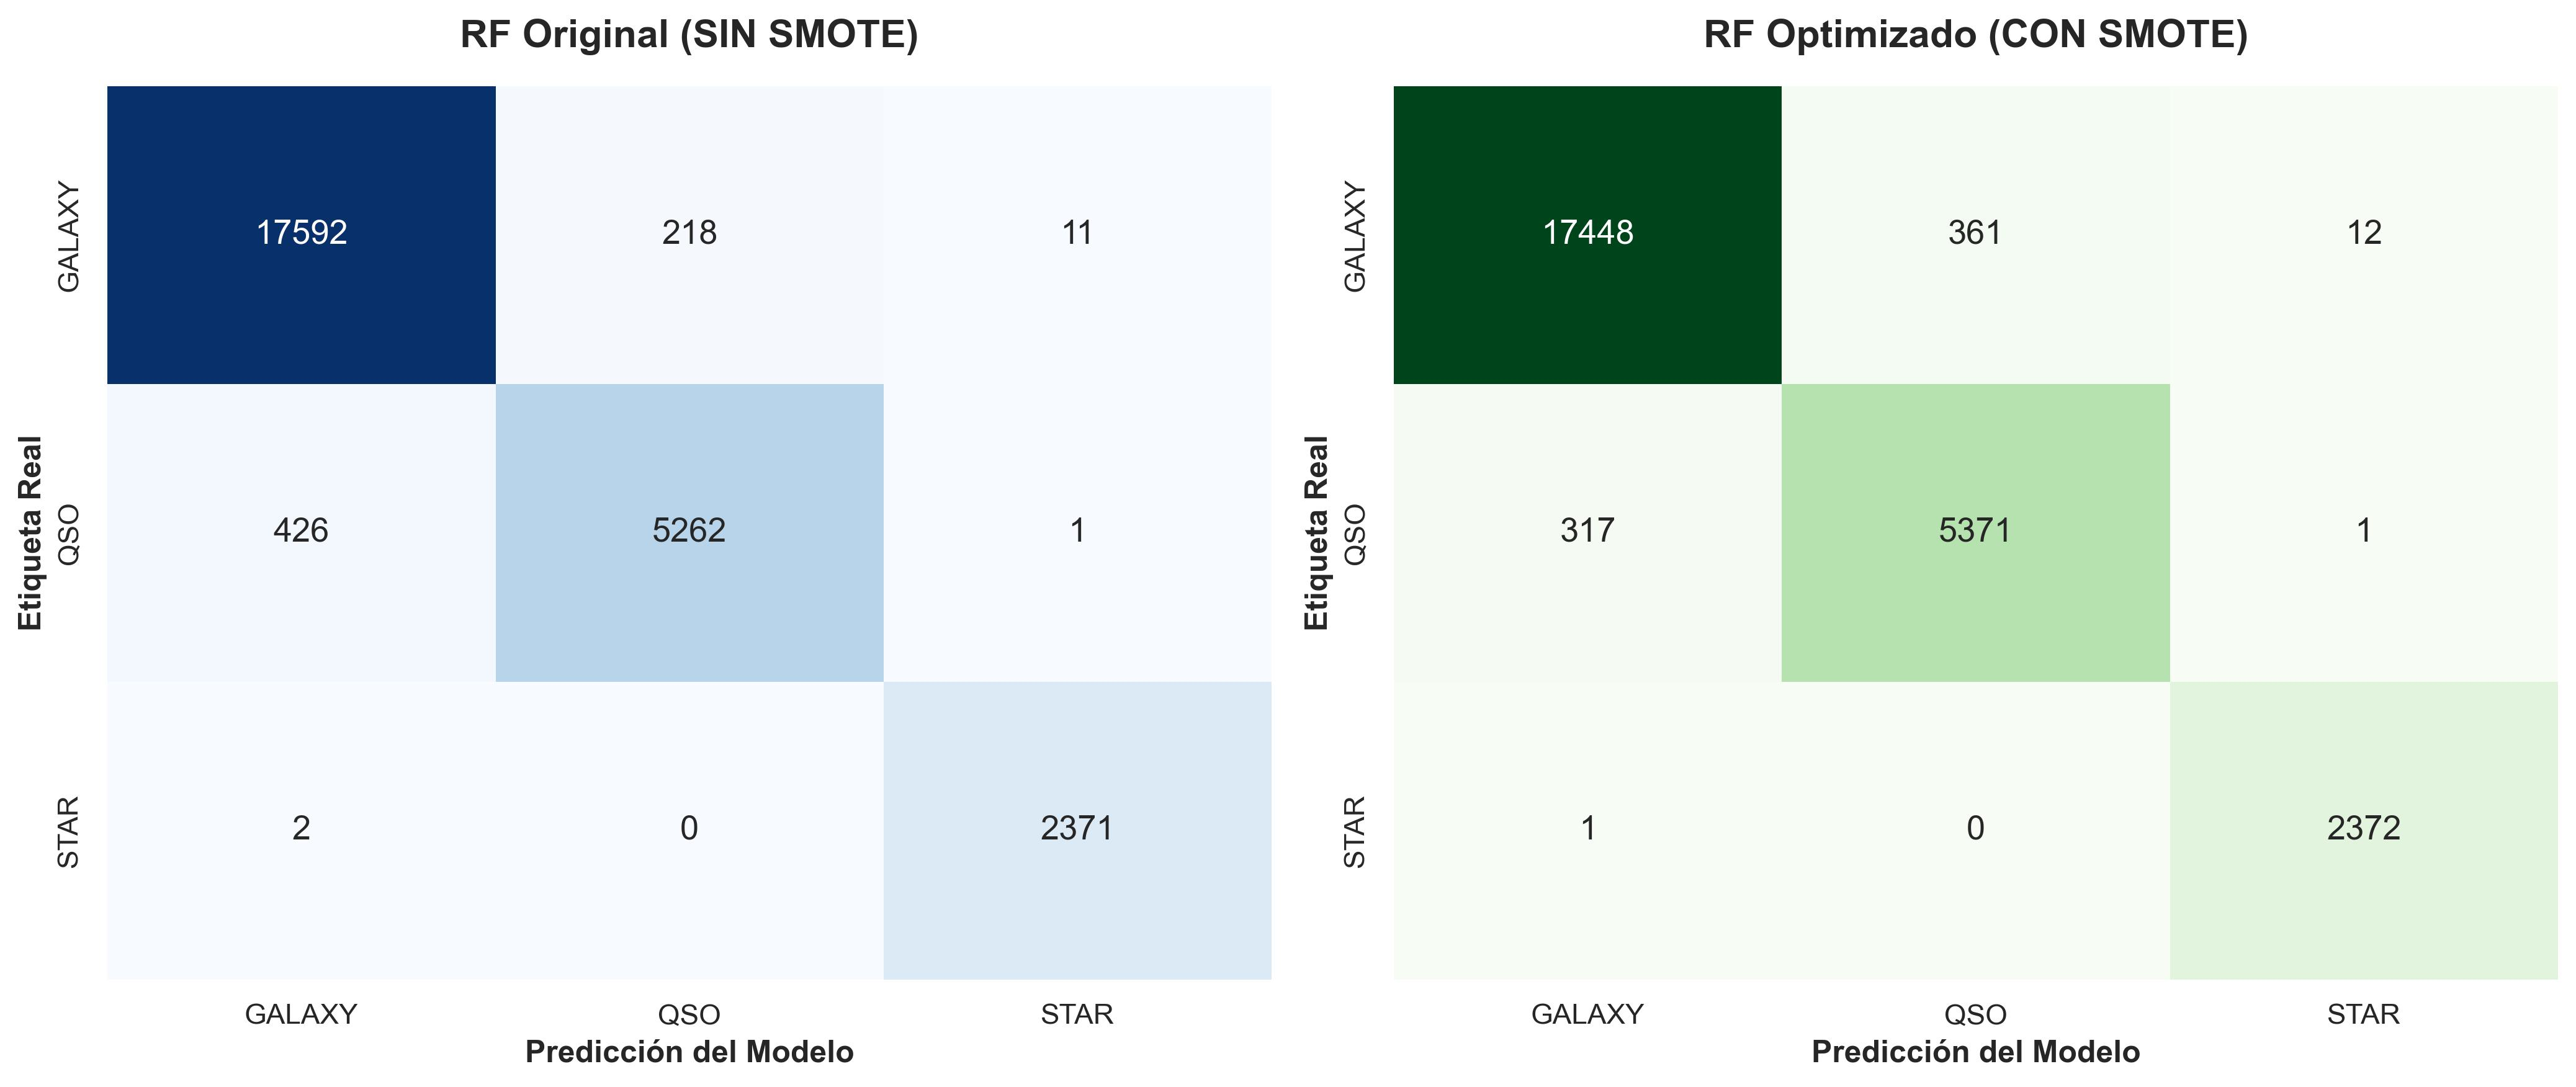
\includegraphics[width=\textwidth]{15_resultado_final_fase4.jpg}
    \caption{Matrices de confusión comparativas evaluadas sobre el conjunto de prueba puro. A la izquierda, el modelo Random Forest original entrenado con datos desbalanceados. A la derecha, el modelo optimizado tras aplicar SMOTE exclusivamente en la fase de entrenamiento. Se observa cómo el balanceo estructural mitiga el sesgo hacia la clase mayoritaria (Galaxias), reduciendo significativamente los falsos negativos en la clase cuásar (\textit{QSO}) y aislando de forma casi perfecta la clase estelar minoritaria (\textit{STAR}).}
    \label{fig:resultados_finales}
\end{figure}

Como se evidencia en la Figura \ref{fig:resultados_finales}, el impacto estructural de SMOTE resultó especialmente notable en la clasificación de los Cuásares (\textit{QSO}). Los resultados de la evaluación arrojaron las siguientes observaciones clave:

\begin{itemize}
    \item \textbf{Recuperación de la clase QSO:} Se logró una reducción significativa de los falsos negativos en la detección de cuásares. El modelo optimizado corrigió la tendencia inicial a clasificar erróneamente estos objetos con exceso ultravioleta como si fuesen galaxias estándar, aumentando sustancialmente su tasa de verdaderos positivos.
    \item \textbf{Estabilidad en la clase Estelar:} De forma paralela, el algoritmo mantuvo una capacidad casi perfecta para aislar la clase minoritaria \textit{STAR}, incurriendo en un único error de clasificación sobre una muestra total de 2373 observaciones estelares (\textit{Recall} de 0.9995).
\end{itemize}

Si bien la exactitud global (\textit{accuracy}) se mantuvo estadísticamente estable en torno al $97.5\%$, la capacidad del modelo predictivo para recuperar objetos de clases minoritarias (fundamentalmente cuásares) mejoró drásticamente. Este hallazgo valida de forma fehaciente la necesidad de implementar técnicas de remuestreo sintético al procesar catálogos astronómicos masivos, los cuales presentan, por su propia naturaleza cosmológica, un fuerte desbalanceo poblacional.


%---------------------------------------------------------------------
% CAPÍTULO 5
%---------------------------------------------------------------------
\chapter{Conclusiones y Líneas de Trabajo Futuro}
\label{chap:conclusiones}
%---------------------------------------------------------------------

El presente Trabajo de Fin de Grado ha abordado el desafío analítico de la clasificación automatizada de objetos celestes (galaxias, estrellas y cuásares) mediante técnicas de aprendizaje automático (\textit{Machine Learning}). Para ello, se ha operado sobre un espacio de características fotométricas multidimensional ($d=5$) derivado de los datos del \textit{Sloan Digital Sky Survey} (SDSS), el cual presentaba un severo desbalanceo poblacional inherente a las metodologías observacionales de cielo profundo.

A lo largo de los capítulos precedentes, se ha dado cumplimiento sistemático a los cuatro objetivos principales planteados en la Introducción (Capítulo \ref{chap:intro}). En primer lugar, se ha validado empíricamente la necesidad de realizar una ingeniería de características basada en principios astrofísicos, demostrando que la transformación de magnitudes aparentes a índices de color es imperativa para cancelar la degeneración espacial y revelar las propiedades térmicas e intrínsecas de las fuentes emisoras.

En segundo lugar, se ha llevado a cabo una evaluación comparativa exhaustiva del rendimiento de dos modelos algorítmicos de aprendizaje supervisado con arquitecturas geométricas contrastadas: por un lado, \textit{Random Forest} (cuyas reglas de decisión trazan particiones ortogonales en el espacio) y, por otro, las Máquinas de Vectores de Soporte o \textit{SVM} (cuyo kernel RBF ajusta fronteras continuas basadas en la maximización de márgenes suaves).

En tercer lugar, se ha investigado en profundidad la viabilidad del aprendizaje no supervisado explorando la topología de los datos en ausencia de etiquetas reales. Para este propósito, se emplearon dos enfoques analíticos: el Análisis de Componentes Principales (PCA) como técnica de reducción de dimensionalidad y visualización, y el algoritmo de agrupamiento K-Means (optimizado estructuralmente mediante la inicialización probabilística K-Means++). Esta aproximación ha permitido demostrar matemáticamente que las clases astronómicas forman un continuo topológico inseparable mediante distancias euclídeas puras, confirmando que la separación observada en ciertos estudios previos depende críticamente de la inclusión subestimada de la variable espectroscópica \textit{redshift}.

Finalmente, se ha logrado optimizar de forma exitosa la detección de las clases minoritarias mediante la implementación estricta de técnicas de remuestreo sintético continuo (SMOTE), mitigando el sesgo estructural impuesto por la clase mayoritaria sin sacrificar la capacidad de generalización global de la arquitectura predictiva.

A continuación, se exponen de forma detallada las conclusiones derivadas de la experimentación, estructuradas en dos bloques fundamentales: por un lado, las implicaciones puramente estadísticas y algorítmicas extraídas del comportamiento de los modelos; y por otro, la interpretación astrofísica subyacente a dichos resultados topológicos.

\section{Conclusiones Estadísticas y Algorítmicas}

Desde el punto de vista de la Ciencia de Datos y la Estadística, los resultados arrojan luz sobre la topología del espacio de color astronómico:

\begin{enumerate}
    \item \textbf{Topología No Convexa de los Datos:} El fallo sistemático del algoritmo K-Means (Sección 4.3) demuestra que las clases astronómicas no forman cúmulos convexos o isotrópicos en el espacio de características fotométrico.
    \begin{itemize}
        \item La proyección PCA reveló que, sin la variable de distancia (\textit{redshift}), las clases forman una distribución espacial conexa con solapamiento no lineal.
        \item Esto invalida el uso de métricas de distancia Euclídea simple para la segmentación no supervisada en este dominio específico.
    \end{itemize}

    \item \textbf{Fronteras de Decisión Ortogonales vs. Suaves:} La superioridad del modelo \textit{Random Forest} (97.8\%) sobre \textit{SVM} con kernel RBF (96.1\%) sugiere que las fronteras de decisión óptimas en este espacio de fases son ortogonales a los ejes.
    \begin{itemize}
        \item Físicamente, esto tiene sentido: los cortes de color suelen ser umbrales estrictos (ej. $u-g < 0.5$).
        \item Los árboles de decisión modelan estas particiones ortogonales de forma nativa, mientras que el SVM intenta ajustar hipersuperficies suaves que, aunque robustas, no capturan con la misma fidelidad las transiciones abruptas entre clases estelares.
    \end{itemize}

    \item \textbf{Eficacia del Remuestreo en la Densidad de Probabilidad:} La aplicación de SMOTE modificó la función de densidad de probabilidad empírica de la clase minoritaria (Estrellas) en el conjunto de entrenamiento.
    \begin{itemize}
        \item Al interpolar sintéticamente, SMOTE ``llenó'' los huecos en la distribución de la clase estelar, permitiendo al clasificador construir una frontera de decisión más generalizable.
        \item Esto se tradujo en un aumento del \textit{Recall} del 0.89 al \textbf{1.00}, eliminando el sesgo de la clase mayoritaria sin introducir un sobreajuste significativo (la precisión global se mantuvo estable).
    \end{itemize}
\end{enumerate}

\section{Conclusiones Astrofísicas}

Desde la perspectiva del dominio de aplicación, los hallazgos validan hipótesis físicas fundamentales:

\begin{enumerate}
    \item \textbf{El Índice de Color como Proxy Físico:} El análisis del espacio fotométrico (Sección \ref{sec:ingenieria_caracteristicas}) confirmó que los índices de color, especialmente aquellos que involucran la banda $u$, poseen el mayor poder discriminante. Esto corrobora que el exceso ultravioleta (originado por la emisión no térmica del disco de acreción en los cuásares) es una propiedad intrínseca detectable fotométricamente, independiente de la degeneración por distancia cosmológica.

    \item \textbf{La Variable de Confusión (Redshift):} El experimento de control demostró que el \textit{redshift} actúa como una variable de confusión en los análisis no supervisados. Su omisión colapsa la separabilidad de las clases, lo que confirma la necesidad de métodos supervisados no lineales para catalogaciones puramente fotométricas.

    % --- NUEVO PUNTO PARA ALARGAR Y DAR CONTEXTO DE BIG DATA ---
    \item \textbf{Escalabilidad para Cartografiados de Próxima Generación:} La consecución de una exactitud cercana al 98\% utilizando exclusivamente un vector de características tabulares ratifica la escalabilidad de los modelos basados en particiones ortogonales. En el contexto de futuros sondeos masivos, como el del Observatorio Vera C. Rubin (LSST) ---que generará catálogos con miles de millones de fuentes---, este tipo de enfoques ligeros ofrece un equilibrio óptimo entre eficiencia computacional y rendimiento científico, permitiendo la pre-clasificación de volúmenes masivos de datos en tiempo casi real.
\end{enumerate}

\section{Líneas de Trabajo Futuro}

Para superar la barrera del 98\% de precisión y abordar las limitaciones detectadas, se proponen las siguientes extensiones:

\begin{itemize}
    \item \textbf{Aprendizaje Profundo (Deep Learning):} Sustituir la ingeniería de características manual por el aprendizaje de representaciones mediante Redes Neuronales Convolucionales (CNNs).
    \begin{itemize}
        \item \textit{Hipótesis:} Una CNN aplicada sobre las imágenes FITS crudas podría extraer características morfológicas (ej. la forma de los brazos espirales o el perfil de brillo PSF) que son invisibles para los modelos basados en tablas de magnitudes.
        \item \textit{Coste Operativo:} No obstante, es imperativo señalar que este enfoque incrementaría drásticamente el coste computacional y las necesidades de almacenamiento, pasando de procesar un espacio tabular ligero a evaluar tensores de imágenes de alta resolución.
    \end{itemize}

    \item \textbf{Inferencia Bayesiana:} Implementar clasificadores Bayesianos para obtener no solo una etiqueta de clase, sino una \textbf{incertidumbre asociada} a cada predicción, algo crucial para la ciencia de precisión.

    % --- NUEVO PUNTO PARA ALARGAR Y DEMOSTRAR VISIÓN DE FUTURO ---
    \item \textbf{Detección de Anomalías para el Descubrimiento Científico:} El presente trabajo ha asumido un universo cerrado de clasificación (Galaxias, Estrellas y Cuásares). Sin embargo, los grandes volúmenes de datos astronómicos suelen albergar objetos peculiares, eventos transitorios raros o artefactos instrumentales.
    \begin{itemize}
        \item \textit{Enfoque Propuesto:} Implementar algoritmos de detección de anomalías (\textit{Outlier Detection}), como \textit{Isolation Forests} o arquitecturas de \textit{Autoencoders} no supervisados. El objetivo sería identificar observaciones que se sitúen en regiones de muy baja densidad del espacio fotométrico, permitiendo automatizar la búsqueda de nueva física que escape a las taxonomías estándar.
    \end{itemize}
\end{itemize}

%---------------------------------------------------------------------
% BIBLIOGRAFÍA
%---------------------------------------------------------------------
\clearpage

\bibliography{bibliografia}
\end{document}
